%%
%% This is file `elsarticle-template-harv.tex',
%% generated with the docstrip utility.
%%
%% The original source files were:
%%
%% elsarticle.dtx  (with options: `harvtemplate')
%% 
%% Copyright 2007, 2008 Elsevier Ltd.
%% 
%% This file is part of the 'Elsarticle Bundle'.
%% -------------------------------------------
%% 
%% It may be distributed under the conditions of the LaTeX Project Public
%% License, either version 1.2 of this license or (at your option) any
%% later version.  The latest version of this license is in
%%    http://www.latex-project.org/lppl.txt
%% and version 1.2 or later is part of all distributions of LaTeX
%% version 1999/12/01 or later.
%% 
%% The list of all files belonging to the 'Elsarticle Bundle' is
%% given in the file `manifest.txt'.
%% 
%% Template article for Elsevier's document class `elsarticle'
%% with harvard style bibliographic references
%% SP 2008/03/01

%\documentclass[preprint,12pt]{elsarticle}

%% Use the option review to obtain double line spacing
\documentclass[authoryear,preprint,12pt]{elsarticle}

%% Use the options 1p,twocolumn; 3p; 3p,twocolumn; 5p; or 5p,twocolumn
%% for a journal layout:
%% \documentclass[final,1p,times]{elsarticle}
%% \documentclass[final,1p,times,twocolumn]{elsarticle}
%% \documentclass[final,3p,times]{elsarticle}
%% \documentclass[final,3p,times,twocolumn]{elsarticle}
%% \documentclass[final,5p,times]{elsarticle}
%% \documentclass[final,5p,times,twocolumn]{elsarticle}

%% if you use PostScript figures in your article
%% use the graphics package for simple commands
%% \usepackage{graphics}
%% or use the graphicx package for more complicated commands
%% \usepackage{graphicx}
%% or use the epsfig package if you prefer to use the old commands
%% \usepackage{epsfig}

%% The amssymb package provides various useful mathematical symbols
\usepackage{amssymb}
%% The amsthm package provides extended theorem environments
%% \usepackage{amsthm}

%% The lineno packages adds line numbers. Start line numbering with
%% \begin{linenumbers}, end it with \end{linenumbers}. Or switch it on
%% for the whole article with \linenumbers.
%% \usepackage{lineno}

\usepackage{multirow}
\usepackage{longtable}
\usepackage{framed}
\usepackage[draft]{ednote}
%\usepackage{ednote}
\journal{Name of Journal here}

\renewcommand{\cite}{\citep}
\newcommand{\citenop}[1]{\citeauthor{#1}~(\citeyear{#1})}

\begin{document}

\begin{frontmatter}

%% Title, authors and addresses

%% use the tnoteref command within \title for footnotes;
%% use the tnotetext command for theassociated footnote;
%% use the fnref command within \author or \address for footnotes;
%% use the fntext command for theassociated footnote;
%% use the corref command within \author for corresponding author footnotes;
%% use the cortext command for theassociated footnote;
%% use the ead command for the email address,
%% and the form \ead[url] for the home page:
%% \title{Title\tnoteref{label1}}
%% \tnotetext[label1]{}
%% \author{Name\corref{cor1}\fnref{label2}}
%% \ead{email address}
%% \ead[url]{home page}
%% \fntext[label2]{}
%% \cortext[cor1]{}
%% \address{Address\fnref{label3}}
%% \fntext[label3]{}

\title{Assisting teachers in an exploratory learning environment
  for algebraic generalisation} 

%% use optional labels to link authors explicitly to addresses:
%% \author[label1,label2]{}
%% \address[label1]{}
%% \address[label2]{}

\author[BBK]{Sergio Gutierrez-Santos}
\ead{sergut@dcs.bbk.ac.uk}
\author[IoE]{Manolis Mavrikis}
\ead{m.mavrikis@ioe.ac.uk}
\author[IoE]{Eirini Geraniou}
\ead{e.geraniou@ioe.ac.uk}
\author[BBK]{Alexandra Poulovassilis}
\ead{ap@dcs.bbk.ac.uk}

\address[BBK]{London Knowledge Lab, Birkbeck}
\address[IoE]{London Knowledge Lab, Institute of Education}

\begin{abstract}
One of the main obstacles to the integration of exploratory learning
environments in the classroom, in spite of their benefits in terms of
student engangement and long-term learning, is the perceived lack of
control by teachers. There is a clear need to provide teachers with
tools that enhance their awareness of the classroom and give them
control over their students' learning activities. 
%
This paper discusses
teachers’ requirements for such tools in the context of an ELE for the
learning of algebraic generalisation and describes our iterative
approach to designing, developing and evaluating them in collaboration
with teachers. We identify the major usage scenarios for the tools and
describe the tools themselves. 
%
The paper also describes the design and outcomes of the formative and
summative evaluations that were undertaken with the tools. We draw
conclusions relating to the value of these tools to teachers and their
possible extensions to other learning domains.
\end{abstract}

\begin{keyword}
     teacher support 
\sep iterative design 
\sep intelligent support 
\sep exploratory learning environments
%% keywords here, in the form: keyword \sep keyword
%% PACS codes here, in the form: \PACS code \sep code
%% MSC codes here, in the form: \MSC code \sep code
%% or \MSC[2008] code \sep code (2000 is the default)
\end{keyword}

\end{frontmatter}

%% \linenumbers

%for reviewing process
%\cleardoublepage

%% main text

\section{Introduction}
\label{sec:introduction}

Exploratory Learning Environments (ELEs) are a particular
type of learning environment where the focus is on students'
exploration of the knowledge domain. Examples of ELEs
include simulators, virtual labs, microworlds, and educational
games. ELEs give considerable freedom to students, who may explore and
learn in a variety of different ways.
%
% ELEs are usually designed to provide opportunities for learners to
% develop conceptual rather than just procedural knowledge in the subject
% domain. 
%
The tasks that students are asked to
undertake are open-ended in nature, may have many alternative
solutions, and encourage students to explore the learning
environment and to follow a variety of solution approaches. Research
has found that considerable guidance is required to ensure learning in
such open-ended contexts~\cite{kirschner06,Kynigos92,MayerDiscovery},
but that in the presence of adequate support ELEs can lead to more engagement
and deeper learning (see~\cite{Noss96,JongJoolingen98} and, for more
recent reviews of the area,~\cite{InquiryLearningJoolingen,Healy2010Charting}). 

In order to provide immediate support to students as they are interacting
with an ELE, recent efforts aim to design intelligent components that 
undertake at least some of the simple aspects of providing feedback to 
students~\cite{MiGen-JRPIT,AmersiConati09}. 
However, this intelligent support cannot completely replace the teacher 
whose role in an exploratory learning setting is that 
of a `facilitator', or `orchestrator'~\cite{Trouche2004,Hoyles2004Integration}. 
This role would be relatively easy in one-to-one student-tutor 
interaction, but scaling it up to the number of students in a 
typical classroom poses several challenges,
that are further compounded by the use technology. 
Given the open-ended nature of the tasks that the students are working on,
teachers can only be aware of what a small number of
students are doing at any one time as they walk around the classroom. 
The computer screens of students who are not in their immediate
vicinity are typically not visible to them and these students may not be engaged
in productive construction (going so far, in our own experience, as
browsing the web, playing games, or engaging in online chat). It is
therefore hard for teachers to know which students are making progress,
which are off-task, and which are in difficulty and in need of additional support.
Even for these students whose screens are currently visible to the teacher, 
it may be hard for her to understand the process by which students have
arrived at the current state of their construction and the recent
feedback they have received from the system, and to provide appropriate
guidance. 

In this paper we present our approach to designing tools that can assist
teachers in a classroom where students are using an ELE. 
Our case study is an intelligent microworld designed to
support 11-14 year old students' development of algebraic ways of thinking. 
We have designed a suite of visualisation and notification
tools, which we refer to as the {\em Teacher Assistance (TA)}
tools. The aim of these tools is to assist teachers in focussing their 
attention across the whole class as students are working with the microworld,
and to inform teachers' own interventions in supporting students to reflect on
their work, on the feedback given them by the microworld and in setting
and working towards new goals. 
% Note from AP: the below is not discussed in this paper, and is more the focus
% of the grouping tool I think:
%,   and in comparing and discussing their
%    solutions with their peers. 

In~\cite{PearceLazard2010Design,IEEE-TLT-TA} we described the architectural design
and implementation of the TA tools, focussing specifically on 
one tool, the Student Tracking (ST) tool (see
Sections~\ref{sec:backgr-relat-work}~and~\ref{sec:teach-assist-tools}~below). 
In contrast, the present paper discusses the pedagogical rationale for
the TA tools, the teachers' requirements from such tools, and the methodological
approaches we have followed in developing them. We identify the main
usage scenarios of the TA tools and discuss the design and results of
a series of formative and summative evaluation activities (these have
only recently been completed and so were not reported
in~\cite{PearceLazard2010Design,IEEE-TLT-TA}).  
Also, the discussion in the present paper encompasses the whole suite of 
TA tools targeted at supporting the teacher in monitoring 
students' activities and progress in the classroom.
 
The outline of the paper is as follows. In
Section~\ref{sec:backgr-relat-work}  we give an
overview of the context and functionalities of our system, and
of related work in the areas of exploratory learning environments and
support for the teacher. In Section~\ref{sec:methodology}
we discuss the methodology we
have adopted in designing, developing and evaluating the TA tools. We
also discuss teachers' requirements from the tools, in the form of
a set of usage scenarios. In Section~\ref{sec:teach-assist-tools}
we describe the tools
themselves --- the Classroom Dynamics (CD), Goal Achievements (GA) and
Student Tracking (ST) tools. Section~\ref{sec:formative-evaluation} 
discusses the formative evaluation of the tools with teachers and 
teacher educators, and changes that were made to them as a result.
Section~\ref{sec:summative-evaluation} 
presents the results from a set of summative
evaluation activities with the tools.
Section~\ref{sec:discussion} discusses the outcomes of these
evaluations. 
Section~\ref{sec:conclusion} 
gives our concluding remarks and directions
for further research.


%%% Local Variables:
%%% mode: latex
%%% TeX-master: "main"
%%% End:


\section{Background and Related Work}
\label{sec:backgr-relat-work}

% REMOVED. IT IS UNNECESSARY (OVERLAPS WITH INTRODUCTION) AND THE
% PAPER IS VERY LONG.
%
% As we mentioned in the introduction, both our group and others have
% made attempts to provide intelligent support in
% ELEs~\cite{MiGen-JRPIT,veermans03,AmersiConati09}.
% However, there will always be situations where the intelligent components cannot 
% help the student or that are intentionally left for the teacher to handle. 
% Examples include very specific conceptual difficulties, 
% engagement nudges to prevent students from getting distracted, 
% and whole-classroom support in, for example, plenary discussions based 
% on students' work. In all these situations, the teacher's role is
% indispensable, especially when dealing with younger children. 
% These types of support are necessary for a productive lesson
% in an exploratory learning setting, yet they can become very
% challenging for the teacher. Depending on
% the classroom configuration, the teacher cannot see all the 
% students' screens at the same time. 
% Even if that is possible, constant demands by the students 
% for the teacher's attention can make it very difficult 
% to monitor what all students are doing at all times. 
% There is therefore a clear need for computer-based support to
% increase the teacher's awareness of the classroom `state' 
% so that she can intervene as appropriate. 
% %In order to design these tools we followed a user-centred approach to
% %derive teacher's requirements in the form of usage scenarios. These
% %are presented in Section~\ref{sec:methodology} whereas the tools are
% %described in more detail in Section~\ref{sec:teach-assist-tools}. 

% In sub-section~\ref{sec:migen-system} we present the MiGen
% system that provides the context in which we have designed and developed 
% a set of Teacher Assistance (TA) tools that aim to assist the
% teacher in focussing her attention across the class and to inform the
% teacher's interventions to support students as they are working in the ELE. 
% We present the MiGen system context in order to help the reader understand 
% our particular case study and to provide a glimpse of the open-ended nature 
% of the activities that students undertake.  In sub-section~\ref{sec:related}
% we present related work.

In sub-section~\ref{sec:migen-system} we present the MiGen
system context in order to help the reader understand 
our particular case study and to provide a glimpse of the open-ended nature 
of the activities that students undertake.  In sub-section~\ref{sec:related}
we present related work.

\subsection{The MiGen system}
\label{sec:migen-system}

The MiGen project (http://www.migen.org) has designed and developed an
intelligent, exploratory environment to support 11 to 14-year-old
students learning of algebraic generalisation.
Using a mathematical microworld called the {\em eXpresser}, students 
are asked to construct two-dimensional tiled models and associated
algebraic rules. In order to build their model, students need to
create `building blocks' out of unit-square coloured tiles depending
on their perception of the model's structure, 
and to repeat each building block in order to form a `pattern'
which forms part of their overall model. 
The algebraic rules they are asked to construct relate 
to the number of tiles of each colour required to paint each 
pattern and their model overall. 
Each building block is made up of a group of
tiles, and can be repeated horizontally, vertically or diagonally to
contribute to the construction of a `pattern'. 
For example, Figure~\ref{fig:example}
shows an example model that students may be asked to construct. 
They may do so by creating building blocks to
generate the centres of the flowers, the petals, and the stalks, 
that they will then repeat to make the yellow, red and green patterns,
respectively. They will be nudged towards deriving rules 
for the number of red tiles and the number of green tiles required 
to paint their model for a given number of yellow tiles.

\begin{figure}[htbp]
  \centering
  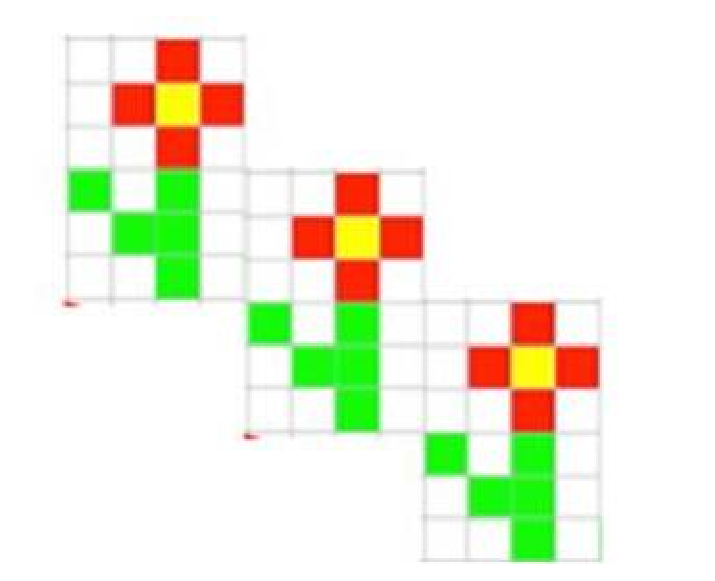
\includegraphics[width=6cm]{gfx/example.eps}
  \caption{An example model that students may be asked to construct in
    eXpresser} 
  \label{fig:example}
\end{figure}

Students are prompted by the eXpresser to check that their models and 
rules are {\em general}, which they can accomplish by making appropriate use of
variables. For example, constructing the model in Figure~\ref{fig:example} requires
one variable --- for the number of yellow tiles. If the model has been
constructed generally by the student, changing the value of this variable
will lead to the whole model being updated correctly and also
still being correctly and fully coloured. The eXpresser has an
`animation' facility which allows students to explore the generality
of their models and rules. This facility automatically applies
different random values to the variables used by the student and
displays the resulting instances of the model in a separate pane of
their screen.  

Tasks are designed to contextualise students' interaction with the
eXpresser and include a set of goals that students need to achieve,
e.g. `construct your model', `make sure it is correctly coloured',
`check that it animates without messing up', and `check that your
animated model is always correctly coloured'. The task goals are
presented to the student within an {\em Activity Document}, in which
students can tick off goals they believe they have completed, answer
questions relating to the task, and reflect on their construction approach.
We refer the reader to~\cite{Manolis2012Sowing} for further 
details of the eXpresser, its `epistemic affordances' and how it can 
enhance students' understanding of algebraic generalisation 
and to~\cite{MiGen-CAE} for further details of the MiGen system architecture, 
the Activity and Task design tools, and Activity Documents.  

Exploratory Learning Environments such as MiGen's eXpresser
have the potential to support students' exploration while at the same
time fostering progressive building of knowledge. However, the
exploratory nature of the tasks undertaken with eXpresser requires
that personalised feedback is provided to students as they construct
their solutions, and not just at the end of the task. This feedback
includes prompts to help students engage with a task, 
guide them towards successful completion of the task, 
and generalise their solutions~\cite{MiGen-CAE,MiGen-JRPIT}. 
This feedback is generated by another
component of the MiGen system, the {\em eGeneraliser}, based on an
analysis of students' actions in the eXpresser. 
% and in MiGen we provide personalised feedback to students as they are
% undertaking their constructions, in the form of a series of prompts
% and nudges that help students reflect upon their interactions and
% guide them towards successful completion of the task. 
%
The aim of the feedback is to balance students' freedom to explore 
while at the same time providing sufficient support to ensure that 
learning is being achieved. We refer the reader to~\cite{MiGen-JRPIT} for
details of the design of the eGeneraliser and of the feedback that it
provides to students. 

%\subsection{Our approach - merge with previous}
%\label{sec:our-approach}
 
%In the MiGen system, 

As students are undertaking the task set in the eXpresser, a series
of {\em indicators} are automatically detected by the eXpresser or
inferred by the eGeneraliser and submitted by them to the MiGen
Server for storage in the MiGen database\footnote{The MiGen software
  comprises the eXpresser running on each student's computer, the TA
  tools running on the teacher's computer, and the MiGen Server and
  database running on a third computer. The MiGen database stores all
  the information produced and required by the eXpresser and the TA
  tools (see ~\cite{MiGen-CAE,IEEE-TLT-TA} for details).}.   
The set of indicators that are meaningful and useful for teachers in
their role in the classroom has been identified through an iterative
process, undertaken collaboratively with our group of teacher
collaborators on the MiGen project (see Section~\ref{sec:methodology}).  

There are two categories of indicators: Task Independent (TI)
indicators refer to aspects of the student's interaction that are
related to the microworld itself and do not depend on the specific task
the student is working on. TI indicators generally refer to a single
action undertaken by the student, such as `placed a tile on the
canvas', `created a building block', `created a pattern'. In contrast,
the detection of Task Dependent (TD) indicators requires 
knowledge of the task the student is working on, may relate
to combinations of student actions, and requires intelligent
reasoning by the system. This reasoning is undertaken by the
eGeneraliser, using a mixture of case-based and rule-based
techniques. Examples of TD indicators are `student has made a
plausible building block for this task', `student has coloured their
pattern generally' and `student has achieved a task goal'. Detailed
discussions of the MiGen's TI and TD indicators and how the latter are
inferred by the eGeneraliser may be found in~\cite{IEEE-TLT-TA}.
 
The TA Tools, described in more detail in Section~\ref{sec:teach-assist-tools},
receive real-time information from the MiGen server relating to
occurrences of TI and TD indicators for each student, and each TA tool
presents a selection of this information in a visual fashion to the
teacher. 
% % REMOVED FOR THE SAKE OF SPACE. SEE ALSO DISCUSSION BELOW (AP NOTE,
% % SG REPLY). 
% % 
% The TA tools include the Student Tracking (ST) tool, the
% Classroom Dynamics (CD) tool and the Goal Achievements (GA) tool. 
% %
% % AP NOTE - N.B. we need enough detail here for the reader to be able to
% % understand Tables 1 and 2, that come before the detailed description
% % of the tools in Section 4! I have added therefore a bit more info
% % here. 
% %
% % SG REPLY - I disagree. I think this is not necessary, so I remove it
% % for the sake of space. Table 1 and 2 are near Section 4, and they
% % actually appear on paper after Section 4 has started. 
% % On a related note, I am not sure Tables 1 and 2 should make
% % reference to the use of the tools... it may be a bit distracting,
% % and overlaps with Section 4.5. 
% %
% The ST tool provides real-time visualisation of the  occurrence of all 
% TI and TD indicators as each student is interacting with eXpresser. 
% Indicators are  coloured Green, Red or Yellow depending on the system's perception
% of whether their occurrence indicates productive interaction,
% unproductive interaction, or interaction that may be productive or
% unproductive depending on context.
% %
% % , showing these in one column of the display for each
% % student, with time increasing downwards, and new information being
% % added at the bottom of the display (see Figure\ref{eee}). Indicators
% % are coloured Green if the occurrence of such an indicator indicates
% % that the actions of the student are consistent with what would be
% % expected by the system from constructive interaction, Red if the
% % occurrence of such an indicator is regarded by the system as an
% % obstruction to constructive interaction, Yellow if the occurrence of
% % such an indicator indicates an aspect of the student's interaction
% % that may be positive or negative depending on the context, and Blue
% % for indicators that represent feedback generated by the system for the
% % student. Further details relating to Figure 2 and the ST tool are
% % given in Section~\ref{sec:4.1}.
% %
% The CD tool represents each student in the classroom 
% visually as a circle whose colour
% is updated to reflect the current status of the student: 
% active (Green), inactive (Amber), or waiting for help from the teacher (Red). 
% %
% % A small subset of the total TI/TD indicators are required to update this
% % information, namely the indicators relating to students'
% % activity/inactivity and students' usage of the eXpresser's help
% % facility. If the teacher clicks on one of the circles in the CD
% % display, that student's current model and rule, as currently being
% % worked on by the student in the eXpresser, is displayed to the teacher
% % (see Figure\ref{fff}).
% % 
% % The teacher can also select to see a summary of the goal achievement
% % information within the CD tool by switching on a feature that displays
% % within the student's circle the number of goals achieved so far as a
% % fraction of the total number of goals e.g. if the student has achieved
% % 2 of a total of 4 task goals, this would show as 2/4� within the
% % student's circle. That feature has been enabled in the display shown
% % in Figure\ref{4r4r}. 
% %
% An optional feature in this tool shows within each student's circle the number of
% goals achieved so far, as a fraction of the total number of goals of the task. 
% %
% The Goal Achievements (GA) tool shows in more detail the progress of each
% student on achieving each of the goals of the task. 
% % 
% % It tracks just one of the indicators - `student has achieved
% % a task goal' - and shows visually, in the form of one row per student,
% % the achievement of each task goal by each student (see Figure
% % 5). Tasks shown as Green are currently achieved, those shown as White
% % are currently not achieved, and those shown as Amber were achieved at
% % some point during the student's construction but are not being
% % achieved by the current model.


%%% End:
\subsection{Related Work}
\label{sec:related}

To our knowledge, MiGen's TA tools represent the first work ---
preliminary results were published in~\cite{PearceLazard2010Design} --- 
targeted at notifying teachers of students' progress and state during
exploratory learning activities in the classroom, notifying the
teacher of students' attainment of key indicators, and aiming to
inform the teacher's own interventions in the class. This novelty of
our TA tools has presented a number of methodological challenges,
which we discuss in Section~\ref{sec:methodology}. 
In the last two years, several similar
initiatives have appeared, including the recent approach
of~\cite{Gutierrez12} ---inspired by early work
in~\cite{Yardi08}--- that focuses on 
informing teachers of students' progress and need for help 
in the context of computer programing labs.
% on progress measurement and
% whether students are stuck in the context of programming labs.
Earlier work (e.g.~\cite{Gueraud09}) focuses mostly on the statistics
 of the interaction (e.g.~how often did the student produce a certain
 kind of indicator). As we discuss in the present paper, our requirements
 analysis with teachers showed that immediate on-line feedback
 about students' current status and progress
 is more valuable to the teacher than simple statistics in supporting the
 `orchestration' of students' use of technologies in the classroom. 
% as it allows orchestrating
% the use of technologies in the classroom.\ednote{MM: I don't understnad
%   the comparison with the statistics --- maybe because I haven't read
%   the work --- also not sure we ever say again what we mean with
%   on-line feedback. Do you mean that the work of Gueraud09 is
%   off-line? SG: Yes.}

The trend towards teacher support is recently growing 
also in the learning analytics community
(see for example~\cite{Crespo12,Zaldivar12,Pardo12}) and there is high
synergetic potential between that work and the work reported here.
Other related initiatives include 
using Web log data generated by course management systems
(e.g.~WebCT) to help instructors become aware of students'
activities in distance learning classes~\cite{Mazza07}; post-analysis of
the system's data logs for helping teachers understand students'
behaviour in adaptive tutorials~\cite{BenAnim08}; 
and providing
awareness information to teachers so as to support their role as 
moderators of multiple e-discussions~\cite{Wichmann09} or class-wide
collaborative activities supported by hand-held devices~\cite{CortezNussbaum2009}. 
%
Particularly interesting is the work described 
in~\cite{Avouris08}, that uses tools to analyse CSCL 
synchronous interaction to help the teacher; their use of ``rules'' to
find specific landmarks in the interaction bears some
similarity to our detection of interaction indicators.  
%
However, none of this work
focuses on exploratory learning activities specifically. 

% Stefan Weinbrenner, Jan Engler, Astrid Wichmann, Ulrich Hoppe
% Monitoring and Analyzing Students' Systematic Behaviour by Agents -
% The SCY Pedagogical Agent Framework. Proceedings of the 5th European
% Conference on Technology Enhanced Learning (EC-TEL 2010), Barcelona,
% ES, 2010

% -- this I think is one of those mentioned at the top
% Stefan Weinbrenner, Jan Engler, Astrid Wichmann, Ulrich Hoppe
% Monitoring and Analyzing Students' Systematic Behaviour by Agents -
% The SCY Pedagogical Agent Framework. Proceedings of the 5th European
% Conference on Technology Enhanced Learning (EC-TEL 2010), Barcelona,
% ES, 2010


% Discussion here also of other related work on: 
% \begin{itemize}
% \item  interaction analysis
% \item  work on CSCL (even if we are not targetting collaboration here)
%   to support teachers 
% \item  work on teachers’ tools for moderating online discussions and
%   argumentation 
% \item  other tools for learning
% \item Argonaut's teacher tools (Astrid Wichman, Ulrich Hoppe)
% \end{itemize}


%%% Local Variables:
%%% mode: latex
%%% TeX-master: "main"
\section{Methodology}
\label{sec:methodology}

In our experience, teachers are not used to having access to tools
such as MiGen's TA tools, and their normal instinct is to walk
round the classroom in order to monitor how individual 
students are progressing and to help them.  
%Indeed, in the first two years of the MiGen project,
%before early versions of the TA tools were available, this was the
%strategy that teachers adopted in helping students who were
%undertaking learning tasks using the eXpresser.  
As discussed earlier,
this approach has significant limitations in an exploratory learning setting
due to the difficulty for the teacher 
to keep track of how a whole class of students are progressing, 
each at their individual pace and using their own
construction approach to the task at hand. Because of teachers'
general lack of experience with tools such as MiGen's TA tools, 
it was not possible for us to elicit from the outset a set of requirements 
for these tools from our teacher collaborators. Instead, it has been
necessary to adopt an iterative methodology comprising
successive phases of prototyping, requirements elicitation,
incremental development and evaluation, in collaboration with teachers. 

%\begin{figure}[htbp]
%  \centering
%  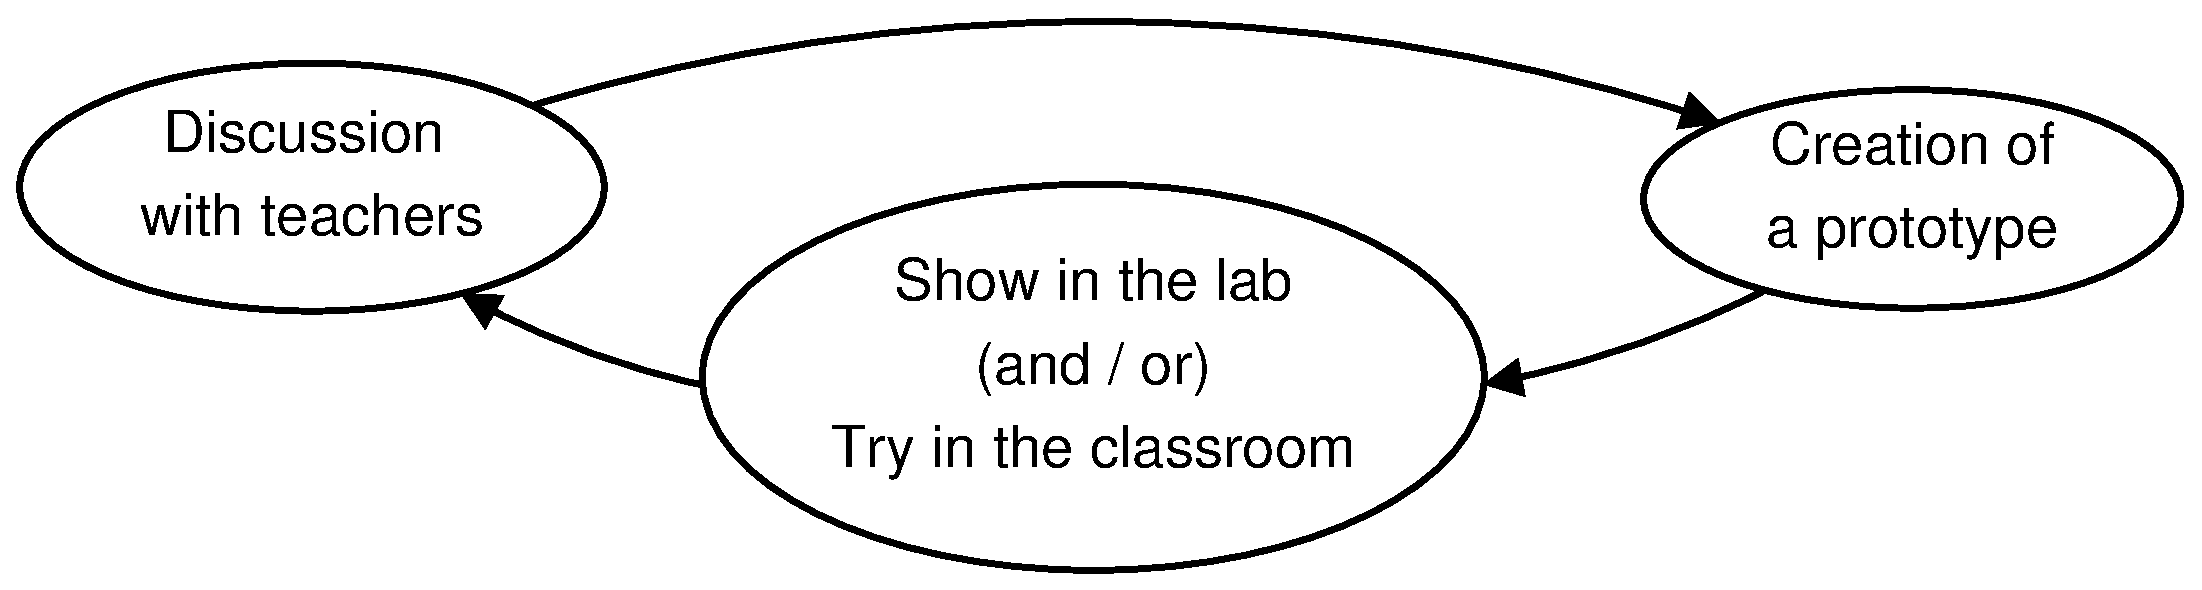
\includegraphics[width=\textwidth]{gfx/methodology.eps}
%  \caption{Iterative design with teachers}
%  \label{fig:it-teachers}
%\end{figure}

%In particular, the development of the TA tools has been undertaken in
%four phases during the course of the project, Phases A - D, which we
%describe below. The number of teachers with whom we have been able to
%collaborate closely during the course of the project is relatively
%small due to practical considerations of the available staff resources
%and the duration of the project. In particular,

Our Teacher Advisory group on the MiGen project comprised around 
20 maths teachers and mathematics educators
from a broad spectrum of secondary schools in the greater London area,
who attended regular project team meetings and gave their input to this 
process. However, the time that these teachers had
available to use early prototypes of the tools in their classrooms was
limited, and collaboration with a core group of 4 teachers
played a prominent role in this respect. 
 
\paragraph{Phase A}
\label{sec:phase-a}

After a first version of the eXpresser and of the student feedback
provided by the eGeneraliser had been developed during the first 15
months of the project, we undertook a first phase of prototyping and
requirements elicitation for the TA tools, working with our teacher
collaborators.    % January 2009 - June 2010
Mockups and
prototypes of several possible visualisations were developed and
discussed in meetings of the Teacher Advisory group and in one-to-one
interviews with those teachers who had trialled the eXpresser and
eGeneraliser in their classrooms. The aim of these interactions was to
elicit teachers' views about what information relating to students'
progress would be useful for them to have as
students are working on eXpresser tasks, and how they would like this
information to be presented.  
As an outcome of Phase~A, two visualisations were developed, 
which subsequently evolved into the Classroom Dynamics
(CD) and Student Tracking (ST) tool (see Section 4 below). 
Also identified were a preliminary set of TI and TD indicators
to be monitored by the system as students are working on the task
set and to be presented to the teacher by the ST tool.

\paragraph{Phase B}
\label{sec:phase-b}

The next phase of development of the TA tools began with several
classroom sessions trialling early prototypes of the ST tool with two teachers
in two schools. % July 2010 - December 2010 
These early trials are described in~\cite{IEEE-TLT-TA} and 
we refer the refer the reader to that paper for details. 
%
%Briefly, the first version of the ST tool was used in
%a classroom trial in July 2010. At that time, only event-based
%indicators were supported by the system, and one of the major items of
%feedback received from the teacher was that some of these indicators
%were actually showing changes in the {\em state} of the student rather
%than being single events, and should therefore be visualised as
%vertical bars in the display that change colour when their status
%changes. This feedback was incorporated into the development of the
%next version of the ST tool. Another major item of feedback from the
%teacher was that the set of indicators displayed by the ST tool should
%be expanded to show also when and what prompts are being generated by
%the system for each student. This feedback too was incorporated into
%the next version of the ST tool.
% 
%In September 2010, a second classroom trial of the eXpresser and ST
%tool was carried out with the same teacher using the new version of
%the ST tool, and also with another of our teacher collaborators in a
%different school. For both sessions, the ST tool was installed on the
%teacher's computer and we observed that the teachers afforded little
%time consulting the tool, spending most of their time in their
%familiar pattern of walking around the classroom to see what students
%were doing and to help them. 
%In post-lesson interviews, the two
%teachers suggested two ways of alleviating this problem: installing
%the Teacher tools on tablet PCs, which would then allow teachers to
%view these tools as they are walking around the classroom; and
%projecting the Teacher tools' display onto the whiteboard at the front
%of the class, again allowing teachers to monitor the progress of
%students as they are walking around the classroom. Both of these
%approaches were adopted for subsequent classroom trials of the system,
%in Phase D.
%
Following the classroom trials, one-to-one
interviews were held with the teachers so as to inform the further
development of the TA tools, and to gain insight into how the
teacher would use such tools in practice in the classroom. 
In these interviews, both teachers suggested that rather than
having the TA tools installed on the teacher's desktop PC, 
it would be preferable to install them
on a tablet PC; this would allow teachers to view the tools as they 
are walking around the classroom without having to keep returning back
to their desk. This approach was adopted 
for subsequent classroom trials of the tools in Phase D. 
% 
%Another major item of feedback received from both teachers was that
%the information being shown by the ST tool was too detailed to be useful to
%them during the lesson. However, they both felt it would be useful to
%be able to track this level of detail for individual students after
%the end of the lesson, for example for those students whose detailed
%progress they needed to check on before planning the next lesson. 
%%As a result of this feedback, we consulted in Phase C 
%%with the pedagogical experts on the project in deriving a subset 
%%of the most significant indicators to be displayed by default in the ST tool. 
%%Teachers can choose to `switch on' more indicators or `swich off' any of this
%%default set by means of an indicator-selection feature. 
%
The need for a third tool was also identified, 
which would show students' incremental achievement of the task goals during the lesson. 
This resulted in the development of the Goal Achievements (GA) tool (see Section 4).  
Finally, a set of Usage Scenarios for the whole suite of tools were identified, 
which we list as US1--US8 in Tables~\ref{tab:UsageScenariosA}
and~\ref{tab:UsageScenariosB}. 
These usage scenarios informed the development of the CD and GA tools,
and the design of the formative and summative evaluations of the 
whole suite of tools in Phases~C and~D. 

\begin{table}[htbp]
  \begin{tabular}{|p{0.5cm}|p{12.5cm}|}
  \hline \multirow{2}{*}{1} & \emph{Finding out which students need
    the teacher's immediate help.} \\
  \cline{2-2} & The teacher can consult the CD tool and see which
  students' circles are coloured Red and how many of the task goals
  they have achieved. The teacher can click on a student's circle to 
  view their current model and rule, to provide some context for the 
  help to be given to the student.
  The teacher can also open up the ST tool to view the
  recent indicators relating to the student's actions, to provide
  additional context. If there is more than one student coloured Red
  in the CD display, the teacher may select to help first students who
  have achieved the fewest task goals. \\
  \hline \multirow{2}{*}{2} & \emph{Finding out which students are
    progressing satisfactorily towards completing the task and which
    students may be in difficulty} \\
  \cline{2-2} 
%  & The teacher can consult the CD tool to see which
%  students' circles are coloured Red. 
%  If there is more than one such student,
%  the teacher may select to help first the students who
%  have achieved the fewest task goals. For any such student, the
%  teacher can click on their circle to view their current model and
%  rule, to provide some context for the help the teacher may then give
%  to the student. The teacher can open up the ST tool to view the
%  recent indicators relating to the students' actions, to provide
%  additional context. 
  & Similarly to US1, the teacher can consult the CD tool to see
  students in need of help, how many task goals students have achieved,
  and students' current models and rules; and the ST tool to
  view students' recent indicators. 
  The teacher can open up the GA tool to view specifically
  which task goals are being achieved by each student. 
  \\
  \hline \multirow{2}{*}{3} & \emph{Finding out which students are
    currently disengaged from the task.} \\
  \cline{2-2} 
  & The teacher can consult the CD tool and see which students'
  circles are currently coloured Amber. If any of these students
  has not completed all the task goals, then she/he is likely 
  to be currently disengaged
  from the task and in need of encouragement from the teacher. If a
  student has completed all the task goals, then she/he may need to be
  set additional goals or a new task to work on while waiting for the
  rest of the class to finish. \\
  \hline \multirow{2}{*}{4} & \emph{Identifying common conceptual and
    procedural difficulties students are facing in order to provide
    more explanation to the
    class as a whole.} \\
  \cline{2-2} 
  & Consulting the GA tool allows the teacher to see which
  task goals students are having difficulty completing, so as to
  inform additional explanation to the class. Consulting the ST tool
  allows the teacher to see if there are specific Red indicators
  showing in many of the students' columns, indicating particular
  procedural difficulties that students may be facing and again
  informing the provision of additional explanation to the class.\\
  \hline
  \end{tabular}
  \caption{Usage Scenarios US1--US4}
  \label{tab:UsageScenariosA}
\end{table}
 
\begin{table}[htbp]
  \begin{tabular}{|p{0.5cm}|p{12.5cm}|}
  \hline \multirow{2}{*}{5}
  & \emph{Finding out which students have finished the task.} \\
  \cline{2-2}
  & The CD tool can be used to see which students have achieved all
  the task goals. For these students, the teacher can click on their
  circles to view their final model and rule, to check if they have
  achieved a correct solution. The teacher can then go to each student
  to set them a new task or additional goals relating to the current
  task, if their solution was correct; or ask them to reflect further
  on their construction if not. \\
  \hline \multirow{2}{*}{6}
  & \emph{Finding out which students have achieved which task goals.} \\
  \cline{2-2}
  & The GA tool can be used to see which students have achieved which
  of the task goals. \\
  \hline \multirow{2}{*}{7}
  & \emph{Providing appropriate support and guidance to individual
  students (i) during the lesson, and (ii) after the lesson.} \\
  \cline{2-2}
  &  % This is a more open-ended use case which 
     This can be undertaken during
  the lesson using a combination of the tools as described for US1,
  US2, US3 above, and after the lesson by using the GA tool to see
  which task goals an individual student has not managed to achieve,
  the CD tool to view the student's final model and rule as produced
  by the end of the lesson, and the ST tool to view the student's
  detailed history of interactions during the lesson.  \\
  \hline \multirow{2}{*}{8}
  & \emph{Reflecting on the class' achievements and planning the next
  lesson.} \\
  \cline{2-2}
  &  % Again, this is a more open-ended use case which can be undertaken by
     % the teacher 
     This can be undertaken using a combination of the GA tool, to see which task
  goals have been largely achieved by the class, the CD tool to view
  selected students' models and rules, and the ST tool to see a
  historical record of how students tackled the task during the
  lesson.
   \\
  \hline
  \end{tabular}
  \caption{Usage Scenarios US5--US8}
  \label{tab:UsageScenariosB}
\end{table}
 
\paragraph{Phase C}
\label{sec:phase-c}

% Phase C of development of the TA tools involved formative
% evaluation of the whole suite of tools with respect to the usage
% scenarios identified from Phase B (Phase C, January 2011 - May 2011). 
This involved formative evaluation of the TA tools, 
firstly with a group of trainee
maths teachers on a Postgraduate Certificate in Education programme
at the University of London, and subsequently with a group of pedagogical 
experts in maths education. We report on the design and outcomes of these 
evaluation activities in Section 5.

\paragraph{Phase D}
\label{sec:phase-d}
 
The final phase of development of the TA tools % June 2011 - February 2012 
involved summative evaluation, undertaken in two parts. 
% In the first part, we conducted a classroom trial in which the
% teacher was first introduced to the TA tools before the lesson, and
% then used them during the lesson as students were working on a
% generalisation task in the eXpresser. 
% The teacher was asked questions
% by a member of the research team during and after the lesson, with the
% aim of evaluating the extent to which the TA tools meet the
% requirements of the usage scenarios. After having used the TA tools in
% one lesson, the same teacher was asked to undertake a similar lesson
% the next day, but this time without referring to the TA tools as she
% attempted to support the students working on a task in eXpresser. The
% aim of this second session was to compare the difference in the
% teacher's experience compared to the first lesson in which she could
% access the TA tools.
In the first part, we conducted two classroom trials, both with the same teacher
and the same class of students. In the first, the teacher had access
to the TA tools to monitor students' progress and support them 
as they were working on a task in eXpresser, whereas in the second  
(held on the next day) the teacher was asked to conduct the lesson without 
referring to the TA tools. 
%
%The second part of the summative evaluation of Phase D involved a
%session held with a new cohort of trainee maths teachers on the
%Postgraduate Certificate in Education programme at the IoE. After
%introducing the eXpresser and TA tools to the participants and
%presenting common ways in which these could be used in the classroom,
%the participants were given access to the TA tools loaded with real
%data from the recent classroom sessions undertaken in the first part
%of the summative evaluation. They were given a questionnaire to probe
%their views about the usage and effectiveness of the TA tools as well
%as specific questions about the classroom status at specific times in
%the lesson, which they had to answer in a limited amount of time -
%simulating in this way the use of the tools in a real classroom.
The second part of the summative evaluation was undertaken with a 
new cohort of trainee maths teachers on the same Postgraduate 
Certificate in Education programme as in Phase C.  
We report on the design and outcomes of these summative evaluation
activities in Section 6.

 

%%% Local Variables:
%%% mode: latex
%%% TeX-master: "main"
%%% End:


\section{The Teacher Assistance Tools}
\label{sec:teach-assist-tools}

As discussed in the previous sections, MiGen's Teacher Assistance (TA)
Tools aim to support the teacher in monitoring students' progress on
tasks set for them to undertake in eXpresser, so that the teacher can
intervene with additional support for the class as a whole or for
individual students as she deems appropriate. 
% , e.g. in providing additional
% guidance, encouraging reflection, or setting new goals. 
% Of course,teachers are very well able to judge what constitutes progress and to
% support their students by appropriate prompts and nudges. As we
% discussed in Section 1, the problem for them is to do that effectively
% with a whole class of students as students are working on exploratory
% learning tasks using eXpresser all at the same time. MiGen's TA tools
% aim to support teachers by reducing their cognitive load and
% increasing their awareness of the classroom `state’.
%
The most detailed tool, and the one developed first chronologically, is the ST tool. 
So we begin with a description of that below, followed by the CD tool and the GA tool.

\subsection{Student Tracking}
\label{sec:student-tracking}

The ST tool monitors the occurrence of TI and TD indicators
generated by each student as they interact with the eXpresser. These
indicators are displayed in chronological order in a top-down timeline for each
student (see Figure~\ref{fig:STtool}), with one column for each student in the
class. Indicators whose occurrence indicates that the actions of the student
are consistent with what would be expected from productive interaction with respect
to the task at hand are coloured Green; indicators whose occurrence is regarded as 
an obstruction to productive interaction are coloured Red; indicators whose 
occurrence indicates that some aspect of the student's interaction may be positive 
or negative depending on context are coloured Yellow; and indicators relating
to feedback given by the system to the student are coloured Blue. 

Timelines can be made thinner or wider using a slider. Using
narrower timelines provides a general overview of all the students' 
timelines but does not show the text associated with the
indicators. Using wider timelines allows a more detailed exploration
of the indicators for a particular student. Timelines can also be made
shorter or longer (so that a vertical pixel represents a longer
or shorter time period). A shorter view allows the teacher to
undertake a general appraisal of all the students' actions so far. A
longer view allows the teacher to look in detail at students' interactions
during a specific time period.
Hovering with the cursor over one of the indicators 
provides further information: full name
of the indicator and precise time it occurred. For some indicators
additional information is also shown, e.g. for the indicator relating
to the accomplishment of a task goal, the full name of the goal. 

Indicators are displayed as horizontal bars or vertical lines
depending on whether they are event indicators or state
indicators. Event indicators relate to an action that happens at a
single time point, e.g. goal accomplished, pattern created, feedback
received. State indicators represent an aspect of the students'
interaction that is always monitored and has a value of `yes', `no' or
`maybe', e.g. `student is active', `student is animating
their model', `a plausible building block is in use'. 
We refer the reader to~\cite{IEEE-TLT-TA} for a detailed description 
of the different categories of event and state indicators. 

The identification of the full set of indicators was achieved through
an iterative process undertaken as a joint activity with our teacher
collaborators during Phases A and B of the project. This resulted in the 
development of computational techniques to track over 50 different indicators. 
However, during the classroom trials in Phase B it became evident that
it was infeasible for teachers to comprehend all of this information
at one time within the ST tool. Larger combinations of the indicators
would be useful for after-class analysis, but the number of indicators
to be displayed during the classroom session needed to be reduced.

The ST tool was therefore extended to allow the teacher to select
which indicators should be shown and which hidden, depending on the teacher's
current needs. For convenience, the indicators are divided into a
number of `families' which the teacher can select to be collectively
shown or hidden (the teacher can also select individual indicators to
be shown/hidden). The families of indicators are: event indicators,
state indicators, building-block related indicators, rule-related
indicators, and important indicators. This last category of `important'
indicators was identified by a team of pedagogical
experts in Phase C of the project (see Section 5 below) 
as being the most relevant for use by the teacher during the lesson. 
The default display of the current ST tool is with this family
of important indicators being shown; teachers can 
choose to `switch on' more indicators or `swich off' any of this
default set by means of the indicator-selection feature. 
The important indicators are all event indicators and
are the following:

\begin{itemize}
        	\item Number unlocked (i.e. variable created), displayed in Green;
        	
		\item Correct/incorrect local rule created (i.e. correct/incorrect allocation 
              of colour in a pattern), displayed in Green/Red;
        	
        	\item Correct/incorrect global rule created (i.e. correct/incorrect allocation
              of colour in the whole model), displayed in Green/Red;

    	    	\item Plausible/implausible building-block created (i.e. probably leads/does not lead
              to a correct solution for the task), Green/Red;
        	
        	\item Pattern made using a plausible/implausible building-block, Green/Red; 
        	
             
        	\item General solution created and animated; displayed in Green if
              the solution animates correctly, otherwise in Red;

        	\item Goal checked by system (i.e. one of the task goals
              has been detected as being accomplished by the system), Green;

        	\item Help requested by the student, Blue; 

        	\item Feedback shown to the student, Blue.

  \end{itemize}
 
Figure~\ref{fig:STtool} illustrates the ST tool visualisation, with the important
indicators and the `Tile placed' indicator selected. 
Looking at the left-most column, we see that student Anne Smith (all students'
names are aliases) has placed a tile, but has then been
detected as being inactive by the system. The system has displayed an appropriate
prompt to the student at this point, and she has resumed placing tiles. 
The system has detected `rhythm' from these tile placements ---
in the sense that the tiles placed on the canvas match part of the target model to
be constructed --- and has suggested that she create a building block from her tiles, 
which she has subsequently done. The system detects that this is a plausible
building block for the task at hand 
(shown by the occurrence of the green `Building Block created' indicator).
Anne continues to create a pattern from her building block, and to accomplish
the first goal of the task. 


\begin{figure}[htbp]
  \centering
  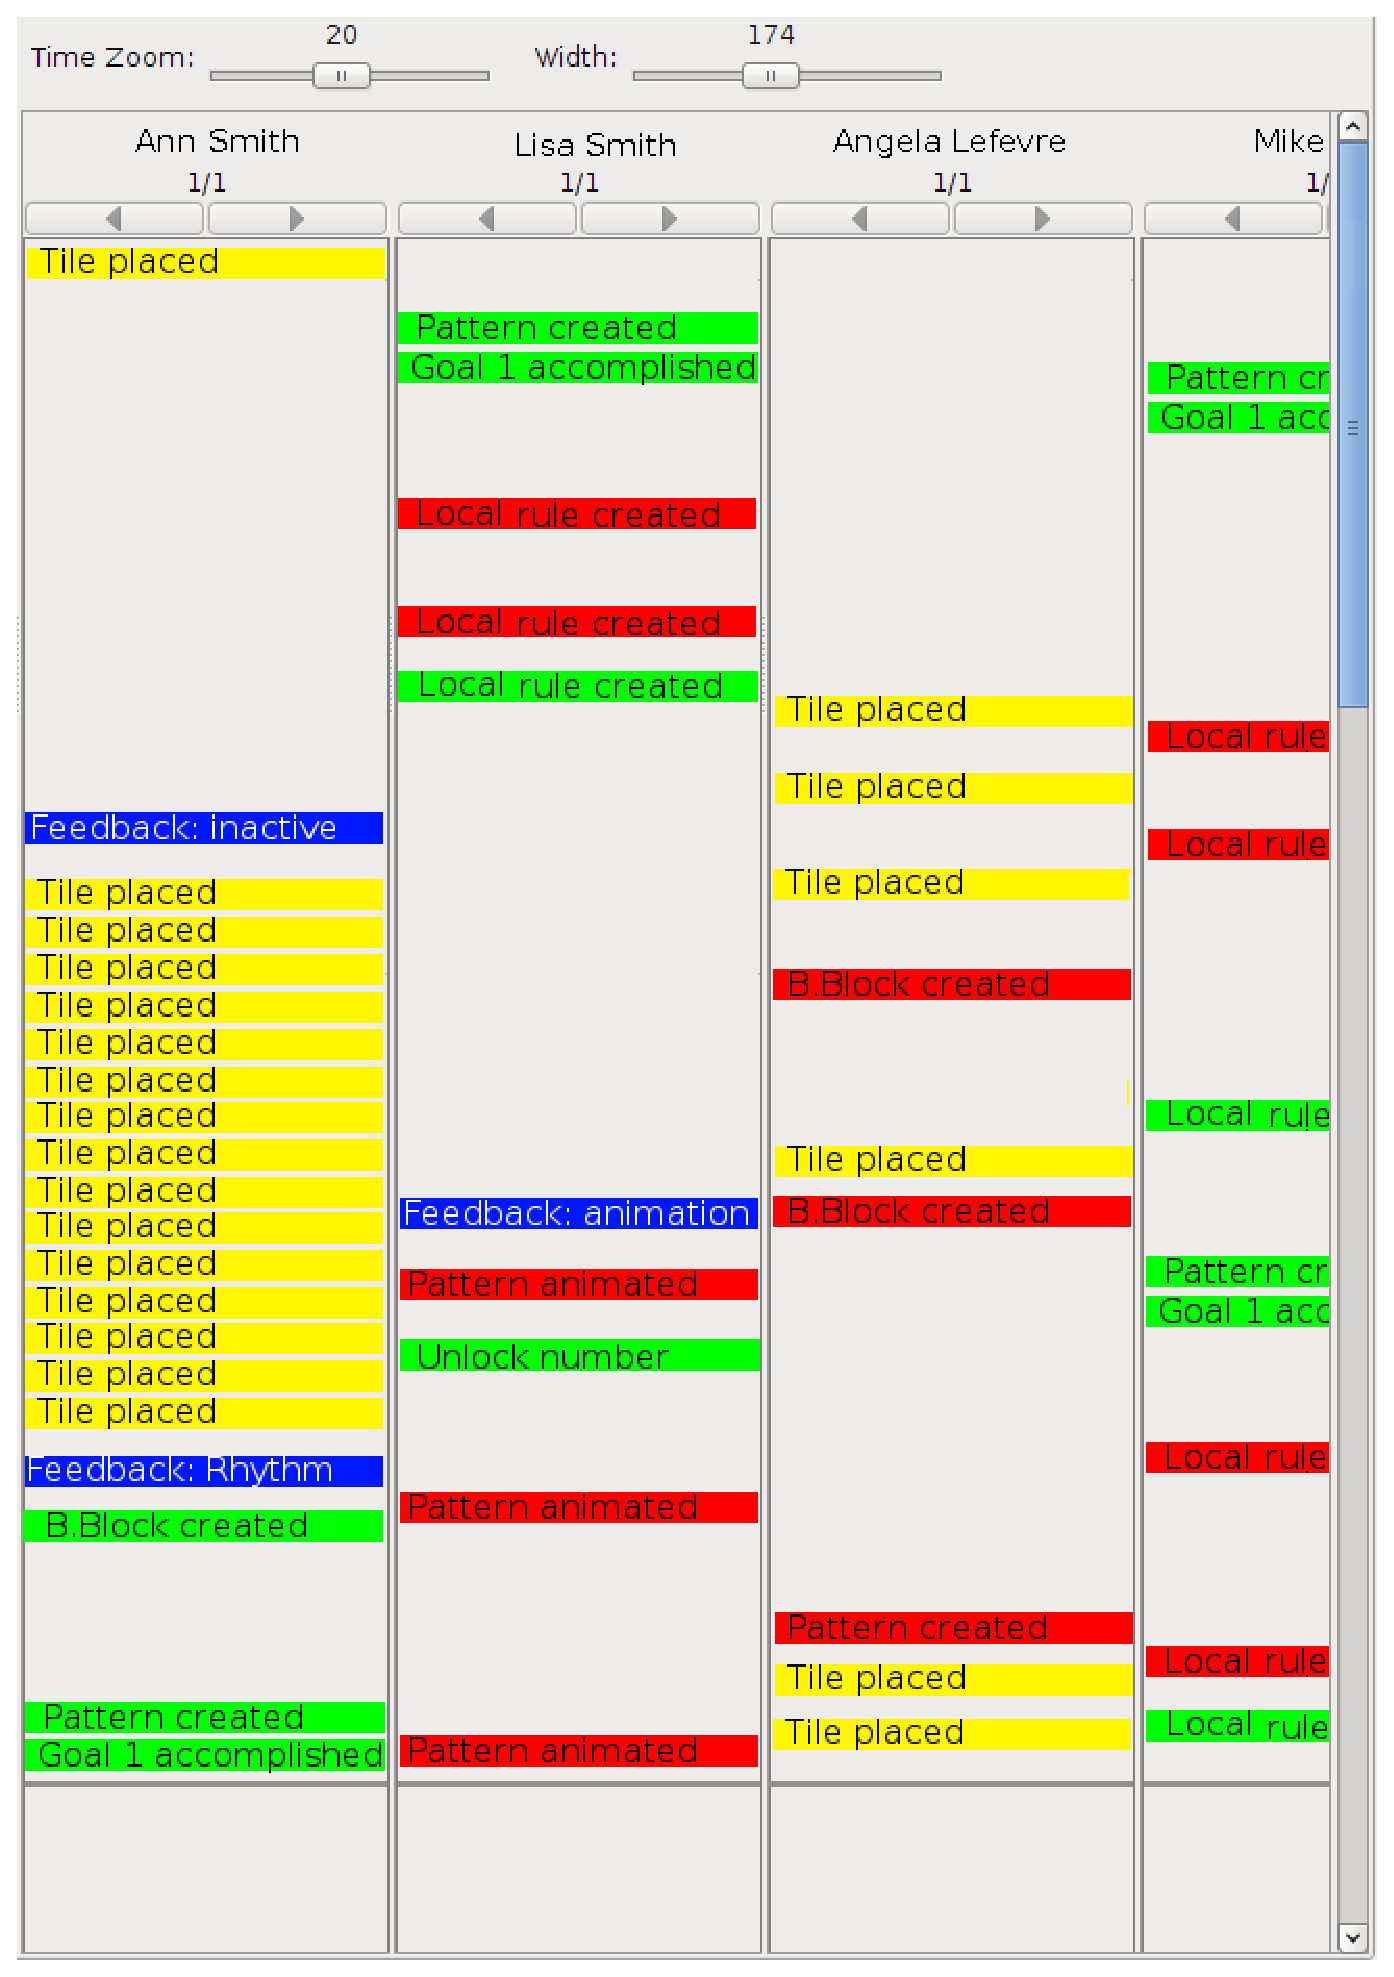
\includegraphics[width=\textwidth]{gfx/ta-st}
  \caption{Student Tracking visualisation} 
  \label{fig:STtool}
\end{figure}

\subsection{Classroom Dynamics}
\label{sec:classroom-dynamics}

The CD tool gives the teacher an at-a-glance overview of which
students are currently engaged with the task and who may be in
difficulty and in need of the teacher's help (see Figure~\ref{fig:CDtool}, left-hand side). 
It represents each student in the classroom by a coloured circle, 
with the student's initials within it.  
Hovering over a circle with the cursor displays the student's full name. 
Clicking on a circle shows the student's 
current construction and current rule (see Figure~\ref{fig:CDtool}, right-hand side). 
The colour of a student's circle reflects the
student's current activity status as perceived by the system:
students shown in Green are working productively on
the task set as far as the system can tell; 
students shown in Amber have not interacted with the eXpresser for some time 
(by default, five minutes); 
%  Unless this is expected by the teacher (for example,
%  sometimes teachers interrupt the lesson to address the class and
%  explain some common misunderstanding), this usually means that the
%  student is distracted, for example talking to fellow student, or
%  playing games in their web-browser.
students shown in Red have requested help from the system
in a situation where the intelligent support cannot help
any further: at such times the eXpresser displays the
message ``The teacher will come to help you now'' 
and the student's circle becomes coloured Red in the CD tool 
in order to attract the attention of the teacher.

\begin{figure}[hbtp]
  \centering
  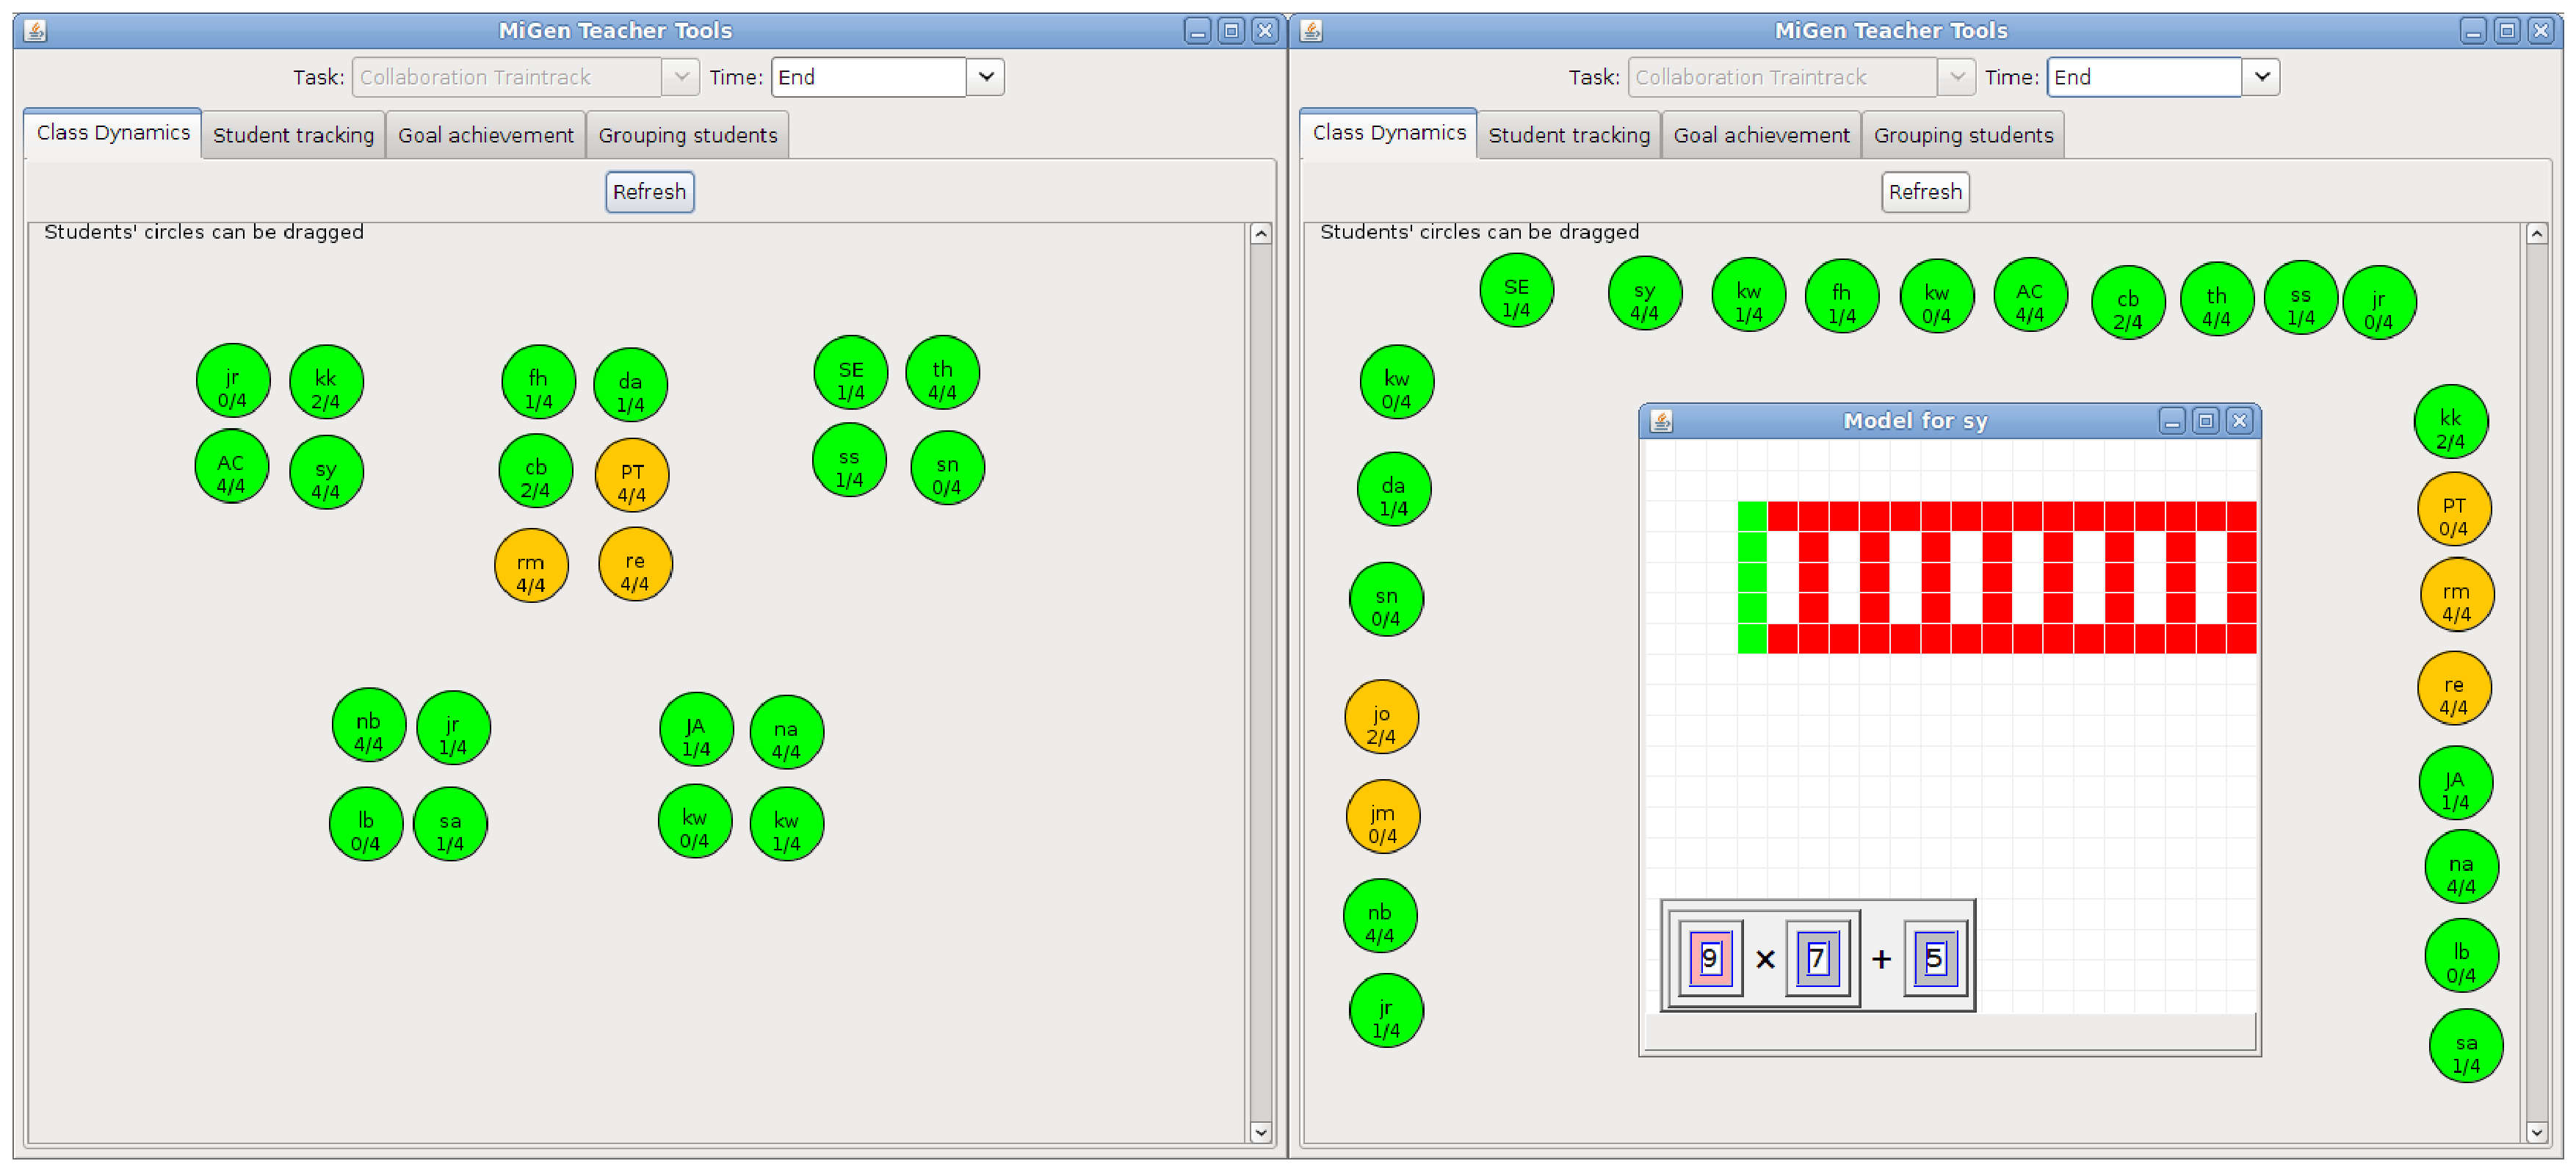
\includegraphics[width=\textwidth]{gfx/ta-cd}
  \caption{Class Dynamics tool}
  \label{fig:CDtool}
\end{figure}

The circles representing the students can be dragged and moved around on
the canvas. This enables teachers to set up the display so that the
position of the circles matches the students'
spatial positioning in the classroom. This helps the teacher to match
the information displayed in the CD tool with her own observations in
the classroom. It also helps the teacher to identify situations that
may be location-dependent. For example, if several students seated at
the same table show as Amber this may indicate that they are
distracting each other and that the teacher should intervene to
refocus their attention on the task.

An optional feature in the CD tool shows within each student's circle the number of
goals achieved so far, as a fraction of the total number of goals of the task. 
For example, if a student has achieved
two of the goals of a task that has four goals, this would show 
as 2/4. This does not provide information about {\em which} of the task goals have
been achieved and generally task goals can be achieved in different
orders. More detailed information about the achievement of task goals
is shown by the Goal Achievement tool. 

\subsection{Goal Achievement}
\label{sec:goal-achievement}

%The Goal Achievement tool shows detailed information about the
%achievement of task goals by students. It allows the teacher to decide
%if more explanation is needed for the class as a whole relating to any
%of the task goals, if a student who has finished the task can be asked
%to help one of the other students, or if the class is ready to move on
%to the next task. 

\begin{figure}[hbtp]
  \centering
  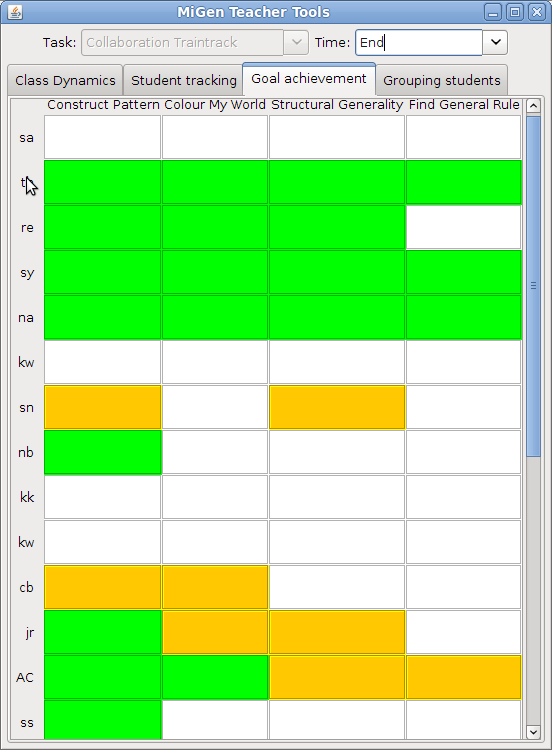
\includegraphics[width=8cm]{gfx/ta-ga}
  \caption{Goal Achievment tool}
  \label{fig:GAtool}
\end{figure}

The GA tool shows a tabular display of students and task goals (see Figure~\ref{fig:GAtool}).
Each row of the table shows the progress of one student (identified by
their initials) in completing the task goals. Each column 
shows the completion status of one task goal for all students. The
names of the tasks are shown at the top and the bottom of the
columns. Each student has several cells next to their name, one
cell for each task goal. Hovering over a cell with the cursor
displays a full description of the goal, the name of
the student and the achievement status of that goal for that
student. We note that the goal achievement information displayed by the GA
tool is inferred by the eGeneraliser and may not necessarily
correspond to the information about goal achievement provided
by the students themselves in their Activity Document: sometimes
students tick as `done' task goals they believe they have achieved
but which the system infers as not actually being achieved;
conversely, sometimes students do not tick as `done' task goals that
the system infers as being achieved.
 
The GA tool uses colour coding to identify the current
status of a task goal for each student:
a White cell shows that a goal has not been achieved yet;
a Green cell shows that the goal is currently being achieved 
by the student's construction; 
an Amber cell shows that the goal has been achieved
by the student during the course of the current task, but is not being
achieved by the student's current construction.
A task goal can appear as Amber for several reasons. For example, some
students may finish the task earlier than others and the system
gives such students the opportunity to undertake the task again but
this time following a different construction approach; such students
would appear with all their task goal cells coloured Amber in the GA
tool and with the cells gradually turning to Green again. 
Some students may not recognise that they have
accomplished a task goal and their further interaction with eXpresser
may result in a situation where the goal is no longer being achieved, 
either accidentally (e.g. a pattern was coloured generally but then a
variable is deleted) or in an explicit attempt to achieve some other
task goal (e.g. in order to relate two patterns via the same
variable, the student may temporarily leave them uncoloured). 
Using three colours for visualising the task goal
achievement information allows the teacher to differentiate between
those students who have moved back and forth taking different
construction approaches to the task and those students who are having
problems completing the task and cannot advance.


\subsection{Time-stop Funcionality}
\label{sec:time-stop-func}

This is a cross-tool functionality provided by all the TA tools. It
allows the user to select a specific point in time, $t$, with respect to
which the ST, CD and GA visualisations are generated. The tools ignore
all indicator occurrences after that time point, allowing analysis of
the situation at that particular time. In particular, the ST tool
shows the history of indicator occurrences for all students up to time
$t$, the CD tool shows the classroom status at time $t$, and the
GA tool shows the goal achievement information at time $t$.  If the
time point selected is in the future, or if no time point is
explicitly selected, the tools show the current situation by default.
 
The time-stop functionality has several important uses. Firstly, it allows
teachers to see information relating to a point in time in the past
in order to better understand the context of a particular situation. 
For example, using the ST tool after the lesson, the
teacher may observe an unexpected sequence of
indicators for a student. The teacher can use the CD tool `frozen'�
at that particular moment to check what was the status of other
students nearby, e.g. were they all inactive/in need of help?
%
Secondly, the time-stop functionality allows the TA tools to be used by
the research team to visualise, for research purposes, the students' 
interaction data arising from each classroom session.
%
Thirdly, being able to use the interaction data gathered from classroom trials 
and to present that data via the TA tools `frozen'�at particular moments in 
time enables the evaluation of the TA tools with a far larger number of teachers than 
those who are able to participate in classroom trials, allowing
the research team to pose questions to evaluation participants 
as if they were in the real classroom at that precise moment. 
%
%Although the situation is not
%identical (the evaluation participants were not under pressure from
%students asking for their help or trying to keep the lesson on track
%while they used the TA tools), having access to a much larger number
%of teachers who could participate in the evaluation of the TA tools
%even if they could not trial the TA tools in their own classrooms was
%extremely helpful in the design and evaluation of the tools, as
%will be discussed below.

\subsection{Example of Use of the TA tools}
\label{sec:example-use}

In order to facilitate readers' understanding of the TA tools, we now 
briefly describe how they may be used in a typical classroom session. 
At the start of the session, the teacher introduces the lesson 
and instructs students to open the eXpresser on their computers and to read
about the current task within the Activity Document. While they 
are doing this, she opens up the TA tools on her computer, typically a tablet. 
For the first few minutes of the lesson, the teacher walks around the classroom 
to make sure that students are focussing on the task at hand and that they
understand the task goals. Once students have begun working on the
task in eXpresser, the teacher can take a step back and use the TA tools to 
help her monitor students' progress. 

Most of the time, the teacher will have the CD tool selected for display. 
If any students show as Amber, she approaches them and encourages them to
resume working on the task. 
%
% The CD tool allows
% the teacher to detect that students that are engaged with the
% computer are not engaged with the learning task at hand: maybe they
% are wasting time on a social network or playing a web game. She does
% not need to see every screen to check student engagement: the CD tools
% does the job.
%
Some students may call out to the teacher for help, or may raise their hands.
The teacher encourages them to first seek help from the system:
``If the system cannot help you, then I will come to you'' she tells them,
knowing that students in such a situation will automatically appear 
red in the CD tool. 
If a student does appear red, the teacher 
goes to the student to help, since she knows that this is a situation where
the system's intelligent support cannot help the student any further. 
If more than one student appears red, she clicks on all those students' cicles 
to see their current models and rules, so that she can prioritise helping 
the students who seem to be having the most difficulty. 

From time to time, the teacher looks also at the GA tool.
Knowing which students have accomplished all the task goals allows
the teacher to set them additional activities.  
Other students may be advancing more slowly; the teacher can use this information to 
set them additional homework so that they can catch up with 
their peers if they need more time than is available in the lesson. 
If the GA tool shows that many students are not achieving a particular task goal, 
the teacher can interrupt the lesson to help all the students at the same
time by clarifying a goal that may be unclear or by providing additional
guidance to help students' understanding.

At the end of the lesson, the teacher can use the ST to examine in detail what 
specific students have done. For example, if the teacher explained during the lesson
to one student how to relate two patterns by using the same variable, 
she can check whether the student started doing this right away or 
required a period of `trial and error' to understand the concept.

%%% Local Variables:
%%% mode: latex
%%% TeX-master: "main"
%%% End:


\section{Formative Evaluation}
\label{sec:formative-evaluation}

During Phase C of the project (January 2011 – May 2011, see Section
3), formative evaluation of the ST, CD and GA tools was undertaken
with respect to the usage scenarios identified from Phase B (the usage
scenarios are listed in Section 3.1). This evaluation comprised two
parts.

The first part was a 3-hour evaluation session undertaken with 26
trainee maths teachers on the Postgraduate Certificate in Education
programme at the Institute of Education in London, split into two
parallel groups of 13 for logistical reasons. Each of the participants
had an installation of the MiGen system running on their computer. In
the first half of the session, participants were introduced to the
MiGen project, the MiGen system as a whole, and the eXpresser
tool. Participants were then asked to work through several
construction examples using the eXpresser so as to gain familiarity
with how students might use it in a lesson and the kinds of feedback
the system would give to students. There was then a 15 minute
break. In the following 30 minutes, each of the TA tools was
introduced to the participants, using real data drawn from one of the
classroom trials undertaken in Phase B of the project. In particular,
using the time-stop functionality, the research team “froze” the
display of the data to a time 10 minutes into the lesson and explained
to participants what could be seen from each tool (these displays are
shown in Figures 2, 3 and 5 in Section 2). For the last hour of the
session, participants were asked to move the display of the TA tools
on their computer forwards, firstly to 30 minutes into the lesson, and
then to 5 minutes before the end of the lesson. For each of these two
time-points, participants were asked to complete a short questionnaire
containing questions relating to usage scenarios US1-US6 – the
questionnaire is listed in Appendix 1. At the end of the session,
participants were asked to complete an end-of-session questionnaire –
also listed in Appendix 1 – relating to the full set of usage
scenarios US1-US8. Two participants never completed this questionnaire
so in the results below we refer to 24 students. The aim of these
questionnaires was to elicit feedback relating to the extent to which
the TA tools met the requirements of the usage scenarios.   
 
We summarise below their answers with respect to each of the usage scenarios.

US 1. Finding out which students need the teacher’s immediate help
 
For both time points (“30 mins before the lesson” and “5 minutes prior
to the end”) most teachers (23/26) answered that they would use the
Class Dynamics tool and look for pupils with red circles. The main
difference between the two scenarios was the level of intervention as
most of the comments related to 30 minutes were about just “keeping an
eye” to certain students who did not seem to have a good start and
ensuring that pupils “marked with an amber are staying focused”
whereas towards the end of the lesson providing help seemed more
critical. 2 responses went beyond using the CD tools and recognised
that “GA also shows levels of progress” and can be used also for
deciding which student needs help. 2 teachers mentioned explicitly the
functionality of clicking on the circles to see what the students have
done and if they are behind group them to help them all together. 
 
With regards to finding out which students need immediate help without
the use of the TA tools, 14 out of 24 teachers answered that they
would use a ‘traditional classroom solution’ e.g. ‘walk around the
classroom viewing students’ work and helping any student who may be
off task or needing help” or “students would have to put their hand up
for my immediate attention”. 8 out of 24 came up with more innovative
solutions like ‘traffic lights’ cards to allow students to indicate if
they are doing well (green card) or might be in trouble soon (orange
card) or definitely need help (red card), cups or even a remote
control that would allow students to ‘call the teacher’. 2 teachers
did not answer at all.

In relation to doing the same task with the tools, 10 out of the 24
demonstrated a deep appreciation of the tools stating that they would
use a combination of the tools starting from the CD tool but also
giving elaborate comments such as “visual review of everyone’s status
helps you really check if students are understanding, without asking
each of them individually”, “allows much faster response to students’
queries” or “It clearly highlights who is active and who isn’t”, “it
also shows what they have been doing which helps as sometimes,
although the student is active, they may not be on task” showing that
beyond the obvious answer of relying on the visualisation of the CD
tool the combination of the tools can provide much more elaborate
information to help decision making. 8 out of 24 provided
straightforward answers such as “simple monitoring such as Class
Dynamics and Goal Achievement give a quick overview” still often
demonstrating that they appreciate the potential of combining
information from different tools. 4 teachers did not answer clearly
but 2 provided simple UI suggestions with the main one (also mentioned
from other teachers especially when providing verbal feedback) being
the suggestion for using the colours in the CD tool to also indicate
goal achievement as additional information that could help in
prioritizing which students need help. 
 
US2. Finding out which students are progressing satisfactorily towards completing the task and which ones may be in difficulty.
 
For this usage scenario, with respect to the 30 minutes into the
lesson situation most teachers (19 out of 26) referred explicitly to
the GA tool e.g. “Students who have yet to achieve any goals are in
difficulty” or a combination of GA tool with CD and ST tools. 5
teachers mentioned only the CD tool as a means of finding out in a
glance which students are progressing (since it provides information
about the number of goals achieved at any given time) and 2 would look
for more detailed information at the ST tool. For the scenario 5
minutes prior to the end most teachers referred to their previous
answer or did not provide an answer. 2 of the 5 teachers who answered
said that they would use the CD tool and 1 mentioned commented that it
would be useful to have the ability to see this information per task
according to predefined expectations that they may have. 
 
With regards to the “end of session questionnaire”, 23 out of 24
teachers recognised again that without the TA tools, they would have
to use again a traditional classroom approach such as “Periodically
ask whole class re stage of progress, level of understanding, Plus
constantly circulate to observe them at work and assist as
required”. 2 of these answers contained a comment about the effort
this would require. One teacher came up with some more innovative
approach: “I could get the pupils to personally fill in a tick box of
how they have progressed, though this would take extra time and
effort.” showing again the difficulty in achieving this in any other
way. In relation to doing the same task with the tools, 13 students
seemed to appreciate how the “tools give you [..] a ‘screenshot’ of
what they have produced.”

US3: Finding out which students are currently disengaged from the task.

For both the “30 minutes” and “5 minutes prior to the end” scenarios
teachers appreciated that they would look for circles coloured amber
and provided answers such as “I would be most concered about amber
students who had yet to achieve any tasks”. Again the difference
between the two scenarios was the level of intervention the would take
as some of them recognises that towards the end of the lesson students
could be disengaged because they have finished with the task and
therefore one approach could be to get “those who have finished to
help those who are still struggling”. Their comments rotated around
their need to be able to configure the timing of disengagement
(something that we introduced later through configuration options) and
ideas for providing more information including the type of
disengagement as it is different to, for example, have the expresser
open and perhaps thinking or discussing with their peers than having
the expresser minimised and being disengaged playing a game or
browsing the internet. They commented therefore that they would have
to observe the class as well and some of them --- both in the
questionnaire and in further verbal feedback they have provided ---
wondered whether it would be possible to show their screens. As there
is relevant software that can achieve this we have not focused on such
a usage scenario but instead feel that the disengagement information
provided by the tool is a first sign for doing exactly as the
participants mentioned, walk around the class and observe who is
disengaged or help them choose which screens to see using additional
software. 



As far as the “end of session questionnaire”, 22/24 participants
answered that without the tools they would use again some traditional
classroom solution e.g. “Periodically ask whole class re stage of
progress, level of understanding, Plus general observation… and
constantly circulate to observe them at work and assist as
required..“. 3 of them commented on the difficulty of this
e.g.“Difficult to keep an eye on all pupils, especially when you are
helping one pupil in particular. Pupils often see you coming and
switch back to task as you approach”. In contrast, 15/24 participants
provided answers that demonstrated their appreciation of the tools in
overcoming these difficulties e.g. “The tools give you a clear
indication of who is currently inactive or has stopped working on
their task for over a minute. This gives you a clear indication of who
might be switching off”. 5/24 provided more elaborate comments
demonstrating that an appreciation also of the transformative nature
of the information provided: “The tools provide a way of helping to
increase the efficiency of my role as a teacher. By enabling me to
look at the student tracking tools and the goal achievement tools I
can readily identify those pupils that appear to be disengaged and
subsequently target them for additional support/ encouragement.” 4
participants did not answer but provided UI and other comments. Most
related to the fact that the disengagement information can be
misleading e.g. “Might highlight pupils who are just having a break to
think [or taking notes]. Also some pupils might be active but just
making up patterns on the program i.e. not sticking to task.” or that
students tend to ‘game the system’ as they can “figure out how to
avoid amber by moving the mouse or dragging and dropping every n
minutes”.   

US4: Identifying common conceptual and procedural difficulties
students are facing in order to provide more explanation to the class
as a whole.  

With respect to this usage scenario we asked on purpose “Would this be
a time-point that you would give more explanation to the class as a
whole? And if so what would you say based on information from the
tools?” for the two time points to see how the participants would use
the tools. From the 17 students who answered this question, 9 referred
to the GA tool and to the white squares that show lack of achievement
of some students compared to the rest of the class, whereas 4 would
rely on the student tracking tool but commented on its complexity
during classroom (another 2 mentioned the CD tool but without any
explanation and 2 did not explain why they would address the whole
class but rather said that they would re-cap and perhaps ask for one
of the students to demonstrate their solution).  Once again, the
difference between the two scenarios was the level of their
intervention i.e. in “30 minutes” within the lesson answers seemed to
be around making sure students are progressing whereas in “5 minutes
prior to the end” teachers were concerned with ensuring that students
have achieved important objectives (e.g. creating expressions) and to
wrap up the lesson . Apart from commenting on the complexity of the ST
tool, other UI improvements involved the scrolling needed for goal
achievement.

For both the “30 minutes” and “5 minutes prior to the end” scenarios
teachers appreciated that they would look for circles coloured amber
and provided answers such as “I would be most concerned about amber
students who had yet to achieve any tasks”. Again the difference
between the two scenarios was the level of intervention the would take
as some of them recognises that towards the end of the lesson students
could be disengaged because they have finished with the task and
therefore one approach could be to get “those who have finished to
help those who are still struggling”. Their comments rotated around
their need to be able to configure the timing of disengagement
(something that we introduced later through configuration options) and
ideas for providing more information including the type of
disengagement as it is different to, for example, have the expresser
open and perhaps thinking or discussing with their peers than having
the expresser minimised and being disengaged playing a game or
browsing the internet. They commented therefore that they would have
to observe the class as well and some of them --- both in the
questionnaire and in further verbal feedback they have provided ---
wondered whether it would be possible to show their screens. As there
is relevant software that can achieve this we have not focused on such
a usage scenario but instead feel that the disengagement information
provided by the tool is a first sign for doing exactly as the
participants mentioned, walk around the class and observe who is
disengaged or help them choose which screens to see using additional
software. 

As far as the “end of session questionnaire” was concerned, 22 out of
the 24 participants answered that without the tools they would use
again some traditional classroom solution e.g. “Periodically ask whole
class re stage of progress, level of understanding, Plus general
observation… and constantly circulate to observe them at work and
assist as required..“. 3 of them commented on the difficulty of this,
e.g.“Difficult to keep an eye on all pupils, especially when you are
helping one pupil in particular. Pupils often see you coming and
switch back to task as you approach”. In contrast, 15 out of the 24
participants provided answers that demonstrated their appreciation of
the tools in overcoming these difficulties e.g. “The tools give you a
clear indication of who is currently inactive or has stopped working
on their task for over a minute. This gives you a clear indication of
who might be switching off”. 5 out of the 24 provided more elaborate
comments demonstrating that an appreciation also of the transformative
nature of the information provided: “The tools provide a way of
helping to increase the efficiency of my role as a teacher. By
enabling me to look at the student tracking tools and the goal
achievement tools I can readily identify those pupils that appear to
be disengaged and subsequently target them for additional support/
encouragement.” 4 participants did not answer but provided UI and
other comments. Most related to the fact that the disengagement
information can be misleading e.g. “Might highlight pupils who are
just having a break to think [or taking notes]. Also some pupils might
be active but just making up patterns on the program i.e. not sticking
to task.” or that students tend to ‘game the system’ as they can “figure out how to avoid amber by moving the mouse or dragging and dropping every n minutes”.  

US4: Identifying common conceptual and procedural difficulties
students are facing in order to provide more explanation to the class
as a whole. 

With respect to this usage scenario we asked on purpose “Would this be
a time-point that you would give more explanation to the class as a
whole? And if so what would you say based on information from the
tools?” for the two time points to see how the participants would use
the tools. From the 17 students who answered this question, 9 referred
to the GA tool and to the white squares that show lack of achievement
of some students compared to the rest of the class, whereas 4 would
rely on the student tracking tool but commented on its complexity
during lessons (another 2 mentioned the CD tool but without any
explanation and 2 did not explain why they would address the whole
class but rather said that they would re-cap and perhaps ask for one
of the students to demonstrate their solution).  Once again, the
difference between the two scenarios was the level of their
intervention i.e. in “30 minutes” within the lesson answers seemed to
be around making sure students are progressing whereas in “5 minutes
prior to the end” teachers were concerned with ensuring that students
have achieved important objectives (e.g. creating expressions) and to
wrap up the lesson. Apart from commenting on the complexity of the ST
tool, other UI improvements involved the scrolling needed for goal
achievement. 

US5: Finding out which students have finished the task

For this usage scenario we asked the participants to provide examples
of students who have finished the task and to provide any comments
they may have. 21 out of the 26 participants who replied to this
question (for both time points) provided correct answers
(i.e. indicated students who have finished the tasks). 13 relied on
information of the CD tool (i.e. the number of goal annotation below
the circles) and the rest on the GA tool. There were not many
additional comments apart from 5 participants commenting on the ease
with which they would check which students have finished the task. One
participant said that close to the end of the class, they would
consider displaying GA information available to the interactive
whiteboard for all the students to see and encourage the ones that are
behind to catch up. With respect to what they would have done without
the tools all participants acknowledge that they would have to revert
to some traditional approach whereby they would ask students who have
finished their task to raise their hands.  

15 out of the 24 answered the related questions in the “end of session
questionnaire”. They  provided answers that demonstrated their
appreciation of the tools. 3/24 participants even provided additional
ideas on how they would take advantage of the GA tool. In particular,
according to their comments, it could help them identify difficult
tasks that they may need to modify or allow them to choose which
students to give extension tasks to. With respect to limitations, the
main requests were for the tool to  take into account “the number of
activities a student has gone through” (probably meaning in a
particular session in order to weight the information provided) and
that students who have completed their task are also somehow displayed
in the CD tool to allow for quick identification and action on behalf
of the teacher (e.g. to be given extension work or to help other
students) 

US6: Finding out which students have achieved which task goals.

The results from this question were very similar to the US5
above. Many students replied “see above”, commented on the intuitive
and simple usage of the GA tool. The only comment worth reporting from
the “end of session questionnaire” was one participant’s confusion
about the three degrees of achievement (i.e. the fact that a goal can
be retracted).  

US7: Providing appropriate support and guidance to individual students
(i) during the lesson, and (ii) after the lesson. 

This is a more open-ended use case which can be undertaken during the
lesson using a combination of the tools as described for US1, US2, U3
above, and after the lesson by using the GA tool to see which task
goals an individual student has not managed to achieve, the CD tool to
view the student’s final model and rule as produced by the end of the
lesson, and the ST tool to view the student’s detailed history of
interactions during the lesson. 


--- CONTINUING WITH THE REST OF THE USAGE SCENARIOS/QUESTIONS  --

Apart from the questionnaires, we also collected teachers’ verbal
feedback and comments during the session. Some of the most important
aspects they mentioned regarding the CD tool include recognising the
value of this tool during lessons compared to the other two tools as
it gave them an instant overview of the whole class’s progress. Some
of them decided to place the circles in an imaginary seating plan,
whereas others grouped them according to their status (e.g. all red
circles together, all green circles together and all orange circles
together). They also made some suggestions to improve the
visualisation of the achieved goals per student in the CD tool. For
example, to have columns made by tiles where each tile represents a
goal or surrounding the circles by an extra layer that gets filled in
parts based on the achieved goals.

Regarding the ST tool, teachers found it quite complicated and not
really useful in lessons. They claimed that it is hard to follow
through what each student did in this view and that they don’t think
they would be interested in all this information. They suggested
instead the idea of deriving a summary of students’ achievements based
on the timelines view. They also asked to be able to see their
students’ current models and rules via the ST tool in a similar way
they can via the CD tool.

Teachers expressed their fondness of the GA tool too and suggested
having all students visible on the screen. For example, instead of
having one long column in which case you need to scroll down to see
the rest of the class, having 2 (or more) columns placed next to each
other would be better to get an instant overview of the whole class’s
progress.

The second part of the formative evaluation was a focus group meeting
held with a group of pedagogical experts in maths education, to obtain
detailed feedback to inform the development of the final versions of
the TA tools, in preparation for summative evaluation in Phase D of
the project. The feedback resulting from this focus group meeting
comprised:

\begin{itemize}
\item Minor visual change requests relating to all three TA tools.
\item A recommendation that all information relating to `state’
  indicators to be turned off, by default, in the ST tool. 
\item The identification of a subset of indicators, comprising the
  most relevant indicators for use by the teacher during a lesson, to
  be displayed by default in the ST tool. 
\end{itemize}

All of the above changes were undertaken by the development team prior
to the summative evaluation of the TA tools. The subset of `important
indicators’ identified by the pedagogical experts are listed in
Section\ref{4.1}.




%%% Local Variables:
%%% mode: latex
%%% TeX-master: "main"
%%% End:


\section{Summative Evaluation}
\label{sec:summative-evaluation}

Phase D of the project (June 2011 – February 2012, see Section 3)
included summative evaluation of the TA tools. This evaluation
comprised two parts. The first part was a classroom-based trial
involving one of our teacher collaborators at her school.  This
teacher had worked closely with us in Phase A and indeed was one of
the teachers who had participated in a classroom trial in Phase B. A
one-to-one session was first held with this teacher where she was
introduced to the final versions of the TA tools, and where she
planned two one-hour lessons that she would undertake with a class of
28 14-year olds using the MiGen system. During the first lesson, the
TA tools were installed on a tablet PC which she carried around the
class with her and consulted as she wished as her students were
undertaking the task set in eXpresser. During the second lesson, which
took place the next day, the teacher did not have access to the TA
tools and had to support the students as they were working with
eXpresser without having access to the information that the TA tools
provide.  During and at the end of both lessons a member of the
research team “shadowed” the teacher and asked her a number of
questions covering between them all the usage scenarios US1-US8, with
the aim of finding out the extent to which the TA tools met the
requirements of the usage scenarios. These questions are listed in
Appendix\ref{rrk}. 
 
*** Analysis of the two sets of responses to the questions is needed
here ****


The second part of the summative evaluation involved a 2-hour session
held with a new cohort of 11 trainee maths teachers on the
Postgraduate Certificate in Education programme at the IoE. Each of
the participants had an installation of the MiGen system running on
their computer. In the first half of the session, participants were
introduced to the MiGen project, the MiGen system as a whole, the
eXpresser, and the TA tools. In particular, the TA tools were
introduced to participants loaded with the real student interaction
data as arising from the classroom trial undertaken in the first part
of the summative evaluation and described above. Participants were
then asked to use the TA tools and the time-stop functionality to
answer a short list of questions relating to usage scenarios US1-US6
at different time points in the lesson. The questions are listed in
Appendix 2 (each relating to a usage scenario). 
Participants were also asked how long it would take them to
answer these questions in the classroom – our aim being not only to
determine if participants were able to use the TA tools to answer the
questions correctly, but how they perceived the amount of time it
would take them to answer the questions in a classroom situation. 

\begin{table}[tb]
  \centering
  \begin{framed}
  \begin{itemize}
  \item Q1. The session started~10’~ago (“10~minutes on”). If you chose a
    student to help immediately, which student(s) would you choose and
    why?
  \item Q2. Based on your experience and previous sessions you would have
    expected by now (“10~minutes on”) that students have achieved at
    least two goals. With a quick glance of the tools would you say
    that the class overall is going according to plan or would you
    intervene and why?
  \item Q3. We are at “30~minutes on”. Based on your experience and
    previous sessions you expected that students would have finished
    by now so that you can progress on the next task. With a quick
    glance of the tools do you think that the class is at that stage
    and why?
  \item Q4. Sometimes students are off-task (e.g. play
    games). At~“30~minutes on”, find two students that are
    disengaged/distracted?
  \item Q5. We are at~“30~minutes on”. Some students need help and you are
    trying to identify others who have finished and can help them. Can
    you give two examples of students who have finished? 
  \end{itemize}    
  \end{framed}
  \vspace{-1em}
  \caption{Questions asked to trainee Math teachers for the summative
    evaluation of the Teacher Assistance tools. Teachers had to answer
    the question and record the time they needed to do so (ranging
    from ``1 -- Very little'' to ``5 -- A lot of time'')} 
  \label{fig:questions-pgce}
\end{table}

All students provided correct examples without any assistance from the
team. The graph shown in Figure~\ref{fig:perceived-time} analyses the
responses relating to the perceived length of time required to
 answer each question. We see, that for all
the questions, no participant responded that they needed a long time
or a lot of time to answer. The questions that were regarded as
requiring the least time to answer were questions 1, 4 and 5, most
likely because they pertain to individual students and could be
answered by consulting just a single tool (the CD tool). Questions 2
and 3 may have appeared to participants as taking more time to answer
because they refer to the classroom as a whole and because, in order
to have a better picture, participants may have consulted the GA tool
as well, and even the ST tool in Question 2 for a more detailed view
of how students are progressing with their constructions. On the
whole, we consider the responses satisfactory particularly as no
answers were perceived as requiring long or a lot of time, which was
our aim. 

\begin{figure}[htbp]
  \centering
    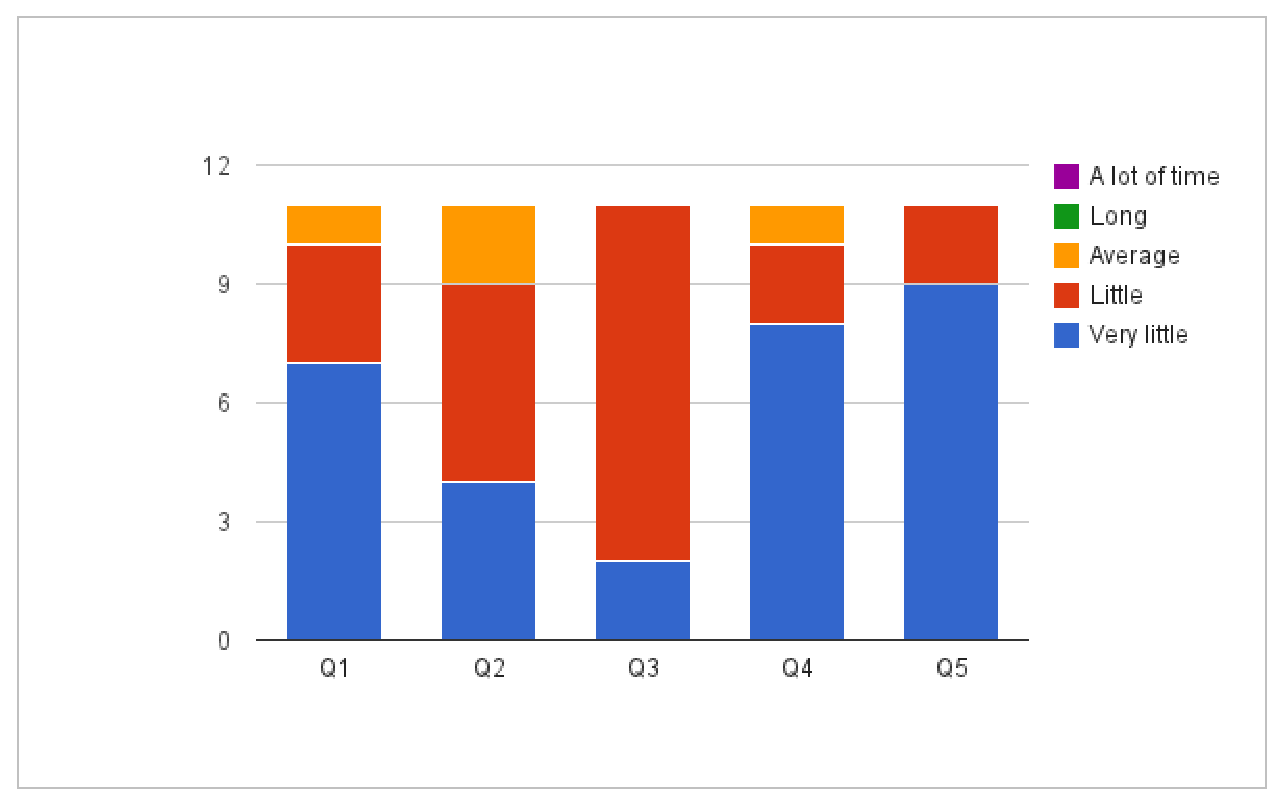
\includegraphics[width=\textwidth]{gfx/perceived-time-Q1-Q5.eps}
  \caption{Participants' perceived time to answer the questions in
Table~\ref{fig:questions-pgce}} 
\label{fig:perceived-time}
\end{figure}


Finally, participants were asked to respond to the following list of
questions, relating to their perceived usefulness of the TA tools for
usage scenarios US1-US8 (where Q1 relates to US1, Q2 to US3, Q3 to
US6, Q4 to US2 and US7(i), Q5 to US7(ii), Q6 to US8, Q7 to US4.) Their
response to each question was selected from 5 choices: Totally Agree,
Agree, Not sure, Disagree, Totally Disagree.

\begin{figure}[htbp]
  \begin{framed}
  I think that the Teacher Assistance Tools (TAT) can help me\ldots
  \begin{enumerate}
  \item \ldots in the
    classroom to find out which students need the teacher's immediate
    help.
  \item \ldots in the classroom to find out which students are
    currently disengaged from the task or distracted.
  \item \ldots to identify which goals have been achieved by which
    students.
  \item \ldots to provide appropriate support and guidance to individual
    students during the lesson.
  \item \ldots to provide appropriate support and guidance to individual
    students and reflect on the class' progress after the lesson.
  \item \ldots to reflect on the class' achievements and to plan for
    the next lesson.
  \item either in the classroom or after the class, to identify common
    conceptual and procedural difficulties students are facing in
    order to prove more explanation to the class as a whole in the
    current or the next session.
  \end{enumerate}
  \end{framed}
  \vspace{-1em}
  \caption{Additional questions asked to trainee Math teachers for the
    summative evaluation of the Teacher Assistance tools (answers
    ranging from ``1 -- Totally Disagree'' to ``5 -- Totally Agree'')} 
  \label{fig:questions2-pgce}    
\end{figure}



\begin{figure}[htbp]
  \centering
    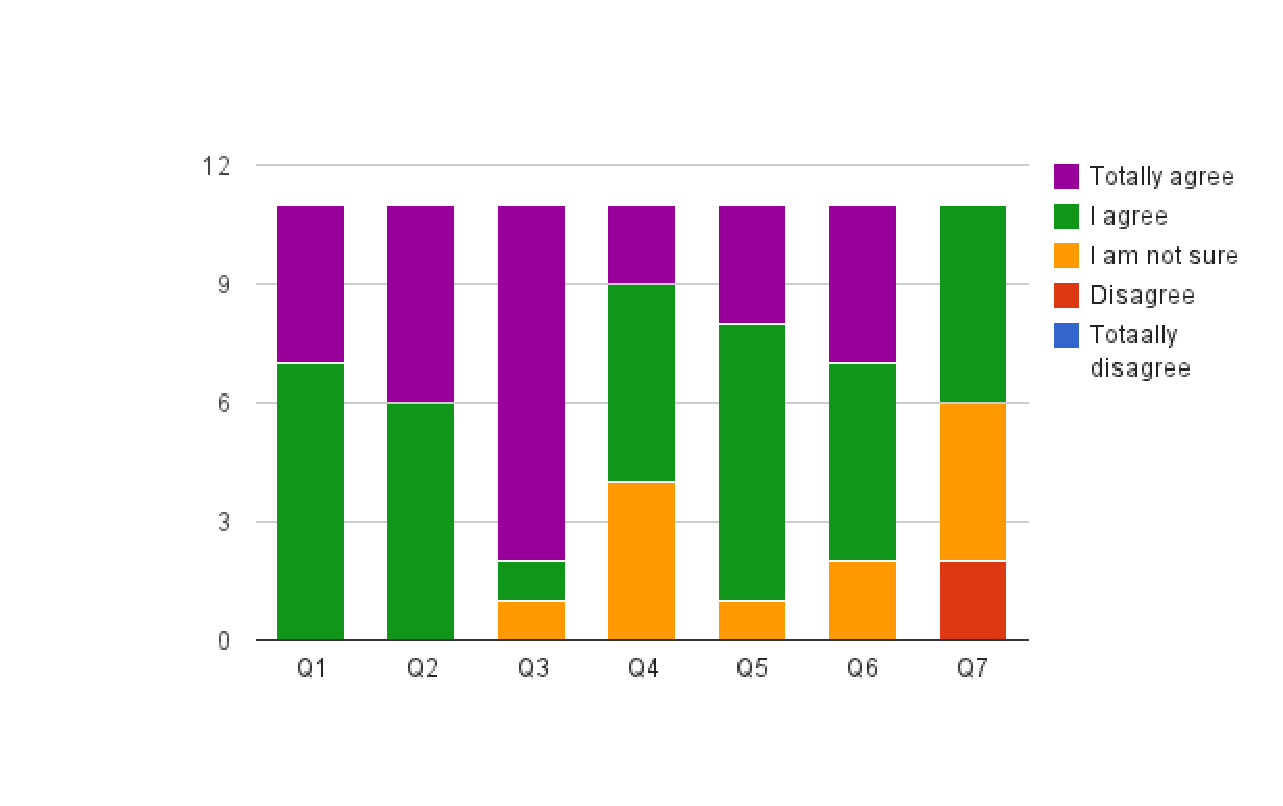
\includegraphics[width=\textwidth]{gfx/agreement.eps}
  \caption{Agreement to the statements in Table~\ref{fig:questions2-pgce}} 
\label{fig:additional}
\end{figure}

Figure~\ref{fig:perceived-time} presents the responses relating to each
question. We 
see that there are no responses of Totally Disagree to any question,
and that only Q7 attracted 2 answers of Disagree. Q1, Q2, Q3, Q5, Q6
had mostly responses of Agree or Totally Agree. Q4 had 4 responses of
Not Sure, and it related to using the tools to inform the provision of
support and guidance to students during the lesson. Q7 had the worst
pattern of responses, with 2 answers of Disagree and 4 answers of Not
Sure, and it related to identifying common conceptual or procedural
difficulties that students are facing. We discuss these results in
more detail in the next Section.




%%% Local Variables:
%%% mode: latex
%%% TeX-master: "main"
%%% End:

\section{Discussion}
\label{sec:discussion}

The results from both the Formative and the Summative evaluations of
the TA tools are encouraging. From the analysis in Section 5 of the results 
of the formative evaluation session held with a cohort of trainee Maths teachers,
we see that participants understood the capabilities of
the tools and were able to use them effectively in answering most
of the usage-scenario based questions. 
The number of responses fell in relation to usage scenarios US4 and US7, 
that concern identifying common conceptual and procedural difficulties
students are facing, 
providing more explanation to the class as a whole, and 
providing guidance to individual students during and after the lesson.
This finding is corroborated by the 
classroom trial held with a teacher at her school, discussed in Section 6,
who reported that answering such questions
required having a global view of the class's `learning status' 
that was difficult to obtain from the tools.
None-the-less, we were pleased to see that a small number of the 
trainee Maths teachers commented that being able to view the occurrence 
of all the indicators in the ST tool does allow teachers
``to identify the most common misconceptions which could then be
consolidated in the following lesson''. 


From the analysis in Section 6 of the results of the classroom trial held with a
teacher in her school as part of the Summative evaluation,
we observed that the teacher was able to use the full suite of TA
tools to address usage scenarios US1, US2, US3, US5, US6, US8 as she undertook a
lesson using MiGen. As noted above, she had difficulty with US4 and US7.
None-the-less, she reported being ``extremely pleased'' with the TA tools. 
One of the main reasons for this seemed to be the experience of control over the class
that she was able to gain using them. With a quick glance at the information being
displayed by the TA tools, this teacher was able to know which students
were making good progress, which students were waiting for her help,
and which students were falling behind with respect to the task goals.
After the subsequent lesson, undertaken without using the TA tools,
she reported that it was not possible to obtain a view
of the class' progress for so many (28) students, 
and that having access to the TA tools during the first lesson 
had made a real difference. 

From the analysis in Section 6 of the second part of the Summative
evaluation, held with another cohort of trainee Maths teachers, 
we see that participants were able to use the tools to provide
correct answers to questions relating to US1--US6 and that no
answers were perceived as requiring ``a long time'' or ``a lot of time''.
In the analysis of the answers to the end-of-session questionnaire,
relating to participants' perceived usefulness of the TA tools, 
only Q7 (relating to usage scenario US4) had any answers of Disagree 
(2 such answers, out of 11 participants); Q7 also had 4 answers of Not Sure.
Q4 (relating to US2 and US7(i)) also attracted 4 answers of Not Sure. 


All of these results point to the usefulness of the TA tools for the
identified usage scenarios. 
None-the-less, the limited number of classroom trials that
it has been possible to undertake given the timescale and resources of
the project, and the difficulties that some evaluation participants
faced in using the tools for the more complex usage scenarios of
identifying common difficulties that students were facing and
formulating their guidance to students, point to the need for
further research, both in attempting to further elicit teachers' needs
from such tools and in undertaking more classroom-based trials.


% We have found that undertaking research in the use of exploratory
% learning environments (ELE) in schools and, specifically, research in
% tools for assisting the teacher is extremely challenging in the
% UK. There are two main reasons for this. First, ELE are not a normal
% part of classroom teaching most schools we have collaborated with. It
% is our impression that the reason for this relates to the need for
% significant support from the teacher in order for ELE to be effective
% in the learning process. As tools such as MiGen that provide
% intelligent support to students as they are undertaking exploratory
% tasks become more common, this situation may change, and teachers may
% be more willing to include use of ELE in their lessons. A second
% challenge we faced was that the use of Teacher Assistance tools such
% as those that MiGen provides is quite new to teachers, and requires a
% change from their usual routine of walking around the classroom to see
% how students are progressing and to provide help on the basis of their
% observations. On the positive side, we have seen evidence in our
% formative and summative evaluations with current and future maths
% teachers that tools such as the ones we have presented here may be
% playing a role in reversing this situation.
% 
% We believe that one of the main factors in the resistance to the use
% of ELE in the classroom is the teacher’s sensation of lack of control
% of the situation: traditional learning is structured in nature, with
% the teacher being in control of the pace and direction of the
% students' learning; in contrast, exploratory environments challenge
% these assumptions. Therefore, tools that can empower teachers by
% making them aware of the `state' of their classroom may serve as a
% bridge that facilitates increased use of ELE in classrooms in the
% future.
% 
 

\section{Conclusion}
\label{sec:conclusion}

In this paper, we have described the iterative development and evaluation of a suite
of Teacher Assistance (TA) tools that target an exploratory learning setting ---
specifically, the learning of algebraic generalisation.
%  --- and
% that aim to help the teacher in enhacing her awareness of the classroom state, 
% monitoring students' progress on the tasks set, and providing support to students. 
In order to design the tools and identify key usage scenarios 
we have collaborated with a number of teacher educators and 
maths teachers in secondary schools in the UK. 
Over the course of the MiGen project, we have conducted several one-to-one, 
small-scale, and whole-classroom trials in a number of 
schools, with 11 to 14-year-old learners and their teachers. 
% It was evident that once our teacher collaborators had used the TA tools in their
% classrooms, they were able to give us more informed feedback and
% influence more clearly the subsequent development of the tools. 

The results of the formative and summative evaluation sessions reported
in this paper show that participants were able to use the TA tools quickly and 
effectively to address usage scenarios US1, US2, US3, US5, US6, US8 ---
concerning teachers' awareness of the classroom state, students' progress 
on achieving the task goals, students in need of immediate help,
and reflection on the class' achievements ---
and that they appreciated the usefulness of the tools for these scenarios. 
There were difficulties in using the tools for usage scenarios US4 and US7 ---
concerning identifying common difficulties
students are facing and formulating their guidance to students. 
None-the-less, a small number of the participants noted 
that the information displayed by the ST tool would 
allow teachers ``to identify the most common misconceptions which could then be
consolidated in the following lesson'', and this is a promising
starting point for further research. 

The development of time-stop functionality across all the TA tools 
allowed us to conduct evaluations of the tools with a far greater
number of teachers (specifically, trainee Maths teachers) 
than those who were able to participate in classroom trials. 
The time-stop functionality allowed us to use real interaction data 
from classroom trials and present it to participants
via the TA tools `frozen' at particular moments in time,  
simulating in this way the experience of using the tools in a real classroom. 
% The situation is of course not identical, as the evaluation participants
% are not under simultaneous pressure from students asking for their help 
% or trying to keep the lesson on track while they use the TA
% tools.\ednote{I think there is no point having the last two sentences
%  and this whole paragraph actually} 

%% Working with teachers and pedagogical experts, we identified early on
%% a key set of interaction indicators that the TA tools needed to track
%% and the ST tool was developed to track this full set. However, during
%% early trials of the ST tool in the classroom, it became apparent that
%% this level of information was generally too detailed to be useful to
%% the teacher during the lesson. Following these experiences, a small
%% subset of indicators that were of most relevance to be tracked during
%% the lesson was identified, and became the default set displayed in the
%% ST tool. Also, the CD tool and the GA tool were co-developed with our
%% teacher collaborators, each of which is based on just a small number
%% of indicators, targeted at providing information about specific
%% aspects of the classroom state.

Based on the teachers' feedback from early classroom trials, we
identified that installing the TA tools on a tablet PC 
helps the teacher to move around the classroom rather than
having to return back to their desk to interact with the tools.
% view the tools, change the tool
% being displayed, focus in on one aspect etc. 
% Our TA tools have been tested and used by teachers on tablet PCs; 
It would be straightforward to adapt the tools to an even smaller screen such
as that of a smartphone and this is an area of ongoing work.
% In one early trial, the teacher decided to also display the 
% Classroom Dynamics tool on the Interactive Whiteboard. The teacher
% reported that this encouraged students to stay on task, as they were
% aware of other students being able to view their progress. 
%%
%% In the classroom trials, we found that the teacher consulted regularly the 
%% Classroom Dynamics tool on the tablet PC. 
%% In this tool, they decided early in the lesson to move
%% the circles representing each student to reflect the seating plan of
%% their class. 
%% As soon as a circle turned red, teachers
%% clicked on the circle to investigate the student's current
%% construction and rule and to prepare an appropriate intervention.
%% Teachers also regularly viewed the Goals Achievement tool during the lesson, to
%% view students' overall progress in terms of task completion. They
%% found this tool very useful when deciding which students to help based
%% on the task goals they had achieved, but also when designing
%% subsequent lessons.
%%
%% One aspect that is worth mentioning is the effect that this kind of
%% \emph{teacher awareness} has on the students. 
%%

In the latest classroom trial, students reacted strongly when the teacher 
told them that she was able to observe from her tablet PC what they were 
doing on their computers. % (some of them quite vocally). 
It was apparent that the sensation of being monitored by the teacher 
led to better general behaviour and more focused work on the part of 
the students. 
We cannot tell without further empirical studies if this 
`better behaviour under vigilance' effect 
would last if the TA tools were used on a regular basis, or whether
students would soon return to their old habits. 
We believe that the effect could be a lasting one if students realised that their
actions would have consequences, e.g. if they did not finish
the task set in the lesson, the teacher would assign them finishing the task
as additional homework, or would take non-completion into account in assessing
their overall performance on this topic. 

We believe that visualisation and notification tools such as MiGen's TA tools 
that are developed specifically to support the teacher in an exploratory learning setting 
in the classroom are better able to provide a sense of awareness for the teacher 
than are general-purpose screen monitoring tools.
% ~\cite{monitor1,monitor2,monitor3,monitor4,monitor5}) 
Screen monitoring tools are not designed for continuous observation 
of the actions of many students during an entire lesson. 
Such tools would require a significant effort
on the part of the teacher to follow and analyse students' actions
comprising clicks, opening and closing of windows, etc. Moreover, such
tools require large screens to be really useful, which is not feasible
during a typical lesson, where the teacher generally needs to be able
to walk round the classroom helping students in addition to using the
tools to monitor the overall classroom state. 
% Although teachers
% usually have a dedicated desk-top computer and often a whiteboard in
% the classroom, our studies in classrooms have shown that teachers
% prefer to interact with the TA tools on a portable device that they
% can carry with them as they walk around the class, rather than being
% required to walk back to their desk at the front of the class in order
% to view a tool, change the tool selected for display, focus in on one aspect etc. 

Our future plans involve research into providing more targeted 
assistance to teachers for the more complex usage scenarios relating to
identifying common difficulties that students are facing and
formulating appropriate guidance for students. We are currently in the
process of sharing the MiGen system with more teachers and
disseminating our results to a wider community. We will continue 
to investigate how such assistance for the teacher
influences the adoption of exploratory learning in the classroom. 

Finally, it is important to note that the TA tools presented in this
paper are general in their design and that such tools could be used to
monitor the activities of students interacting with other exploratory
learning environments provided that the environment 
detects appropriate interaction indicators.
This would need to include as a minimum indicators relating to 
students' current activity status, 
waiting for help from the teacher, and goal
achievement status: 
these are the indicators that drive the CD and GA tool visualisations 
which we have found that, in practice, teachers consult most often during a lesson. 
Our future work therefore involves investigating how the TA tools
could be adapted to support teachers using even more complex
exploratory learning environments (such as that of the Metafora
project (www.metafora-project.org)~\cite{Dragon13}, which focuses on
meta-learning) and beyond that for virtual science labs, medical simulators, 
and interactive environments for novice programmers.

%%% Local Variables:
%%% mode: latex
%%% TeX-master: "main"
%%% End:

\appendix

\section{Formative Evaluation in the Lab, Phase~C}
\label{sec:form-eval-with}

\subsection{Evaluation form}
\label{sec:evaluation-form}

There are the question from the questionnaire form that had to be
filled in by participants, relating to information displayed by the TA
tools using time-stop functionality: (i) 30 minutes into the lesson,
and (ii) 5 minutes before the end of the lesson. For each question or
teacher's task the evaluation subjects had to write down how they
would answer the question using the tools. They could also add their
comments, if any.

\begin{enumerate}
\item Finding out which students need your immediate help
\item Which students are progressing satisfactorily towards completing
  the task goals? Which students may be in difficulty?
\item Which students are currently disengaged from the task?
\item Would this be a time-point that you would give more explanation
  to the class as a whole? And if so what would you say based on
  information from the tools? 
\item Which students have finished the task?
\item Which task goals have most students achieved?
\end{enumerate}

\subsection{Further comments}
\label{sec:further-comments}

At the end of the session, they were given another questionnaire form
in which they had to answer three questions for every question or
teacher's task: (i) How would you find out without using the TA tools;
(i) with the TA tools, (ii-a) if the tools helped you achieve this
task, how did they do it, (ii-b) if they did not, what additional
information would help you?

\begin{enumerate}
\item Finding out which students need your immediate help.
\item Finding out which students are progressing satisfactorily on an
  eXpresser activity and which ones may be in difficulty
\item Finding out which students are disengaged during the activity
\item Identifying common conceptual and procedural difficulties
  students are facing in order to provide more explanation to the
  class as a whole.
\item Providing appropriate support and guidance to individual
  students during the lesson
\item Providing appropriate support and guidance to individual
  students after the lesson
\item Finding out which students have finished the task
\item Finding out which students have achieved specific task goals
\item Pairing students for collaborative tasks
\item Planning the next lesson using the MiGen system
\item Planning the next lesson without using the MiGen system
\end{enumerate}

\section{Summative Evaluation in the Classroom, Phase~D}
\label{sec:summ-eval-classr}

The following questions were posed to the teacher by a member of the
research team, firstly during the first lesson when she had access to
the TA tools and, again, during the second lesson when she did not
have access to the TA tools. The questions were asked at precise
points in time in both cases, as indicated (the lesson lasted 55
minutes). Each question relates to one or more of the Usage Scenarios
described in Section\ref{sec:usage-scenarios}, as indicated in square
brackets.

\begin{description}
\item[Question 1 (15 minutes into the lesson): ] (i)~which
  students are progressing satisfactorily in undertaking the task?
  [relates to Usage Scenario US2], (ii)~which students may be in
  difficulty?~[US2], and (iii)~which students need your immediate
  help?~[US1]
\item[Question 2 (25min): ] for the students that you have chosen to
  help, what guidance did you give each one?~[US7]
\item[Question 3 (35min): ] which students may be disengaged from the
  task? [US3] which students have achieved Task Goal~3?~[US6]
\item[Question 4 (45min): ] what common conceptual or procedural
  difficulties are students facing?~[US4], what explanation might you
  give to the whole class at this time?~[US4]
\item[Question 5 (end of lesson): ] Now that the lesson has finished,
  (i)~which students have finished the task?~[US5], (ii)~what 
  additional guidance might you give to any particular
  students?~[US7], and (iii)~what are your views about the class’s
  achievements in this lesson, plus how might you plan the next
  lesson?~[US8] 
\end{description}



%%% Local Variables:
%%% mode: latex
%%% TeX-master: "main"
%%% End:



\section*{Acknowledgements} 

The MiGen project was funded by the ESRC/EPSRC Teaching and
Learning Research Programme (Technology Enhanced Learning; Award no:
RES-139-25-0381).

\bibliographystyle{elsarticle-harv}
\bibliography{2009-04-28-group-6308,cae-cal09}

%\begin{thebibliography}{00}
%% \bibitem{label}
%% Text of bibliographic item
%\bibitem{}
%\end{thebibliography}

\end{document}

\endinput
%%
%% End of file `elsarticle-template-harv.tex'.


